%!TEX root = ../masters.tex

\chapter{Referencial Teórico}
\label{cha:literature}

O campo de extração de informação vem sendo bastante pesquisado e difundido. Por sua vasta aplicação, vários estudos foram e são desenvolvidos, abrangendo diversos métodos e modelos de extração, que utilizam também de PNL (Processamento Natural de Linguagem) \cite{Sarawagi:2008:IE:1498844.1498845}. 

Visando abranger grande parte da literatura sobre o assunto, alguns eventos e bases de dados importantes foram mapeados para a pesquisa, a fim de encontrar trabalhos relevantes para a área. Foram mapeados:

\begin{itemize}
    \item KDIR (International Conference of Knowledge Discovery and Information Retrieval);
    \item ICDAR (International Conference on Document Analysis and Recognition);
    \item PDCAT (International Conference on Parallel and Distributed Computing, Applications and Technologies);
    \item IAPR (International Workshop on Document Analysis Systems);
    \item ACM Conference on Digital Libraries.
\end{itemize}

Estes eventos foram analisados através da observação de todas as citações e referências utilizadas em cada artigo publicado, bem como outros detalhes importantes para a pesquisa.

\section{Metadados}
\label{sec:metadados}

\subsection{Conceito de Metadado}
\label{ssec:metadata-concept}

Com base nas ideias apresentadas por \cite{meta-dados}, ``[...] um elemento de metadado descreve um recurso de informação, ou ajuda a fornecer acesso a um recurso de informação.''. Todo dado que agregue nova informação a um recurso pode ser considerado um metadado. Quanto mais metadados um recurso tiver, mais detalhado ele é, ou seja, mais dados sobre ele se tem. Podemos simplificar ainda mais a definição de metadado como sendo ``um conjunto de dados sobre um determinado recurso''.

Podemos citar como exemplo a utilização de pequenos pedaços de dados sobre um conjunto de livros, dentro de um ambiente de biblioteca, o que é considerado uma coleção de elementos de metadados \cite{meta-dados}. O mesmo autor também cita como exemplos de metadados os dados coletados por mecanismos de busca no momento em que páginas da Internet são indexadas e então armazenadas.

\subsection{Padrões de Metadados}
\label{ssec:metadata-patterns}

Diante da infinidade de dados que podem estar atrelados a um determinado recurso, temos uma amplitude muito grande de características que podem ser definidas como sendo metadados. Assim, foram definidos 15 (quinze) elementos para descreverem um recurso informacional, estabelecendo então um padrão adotado em todo o mundo, o padrão ``Dublin Core'' \cite{dublin-core}.

Este padrão se originou após uma série de encontros feitos desde 1995, unindo bibliotecários e pesquisadores digitais e de conteúdo, visando identificar padrões para se representar um recurso eletrônico. O nome ``Dublin'' foi dado em virtude da primeira reunião do grupo, que foi realizada na cidade de Dublin, Ohio. Já o nome ``Core'' se deu em virtude dos elementos serem amplos e genéricos, sendo então utilizados para descrever uma grande variedade de recursos.

Os quinze elementos que fazem parte do padrão Dublin Core compartilham de um vasto conjunto de vocabulários de metadados. Suas especificações técnicas são mantidas pela \emph{Dublin Core Metadata Initiative} (DCMI), agência responsável pela definição destes elementos.

Este padrão é utilizado para se representar um recurso na Internet \cite{dublin-core-1-1}. Com base em suas características, mecanismos de buscas podem indexar um recurso de maneira mais rápida e precisa, pois este é acompanhado de pequenas sinalizações sobre seu conteúdo, apresentados em forma de metadados. 

Para cada elemento descrito pelo padrão temos informações como: 

\begin{itemize}
    \item \textit{label}, que é o texto para leitura e entendimento humano;
    \item \textit{name}, que é usado para o processamento de máquina, ou seja, um identificador único que a máquina utiliza para reconhecimento.
\end{itemize}

Os elementos que fazem parte da versão 1.1 do padrão Dublin Core \cite{dublin-core-1-1} podem ser vistos no \refanexo{attach:dublin-core} deste trabalho.

Abaixo podemos ver um exemplo de código para utilização de metadados Dublin Core em uma página da Internet, onde iremos referenciar os elementos \textit{creator}, \textit{title} e \textit{language}.

\lstset{language=HTML}
\begin{lstlisting}[escapechar=\#]
<meta name="DC.Creator" content="#\imprimirautor#" >
<meta name="DC.Title" content="#\imprimirtitulo#" >
<meta name="DC.Language" content="pt_BR" >
\end{lstlisting}

A indexação do autor (\textit{DC.Creator}) da página, bem como seu título (\textit{DC.Title}) e idioma (\textit{DC.Language}), são feitos de maneira bem simplificada e direta. Para páginas da Internet, com as informações todas em formato HTML, a utilização destes metadados perderia o sentido, visto que essas informações poderiam ser facilmente encontradas de outras formas, como a análise do próprio código. Para documentos binários - em formato PDF ou Word, por exemplo - a utilização destes metadados é de suma importância, visto que permite que essas informações básicas sejam capturadas sem a necessidade de análise do conteúdo destes arquivos.

\subsection{Técnicas de Extração de Metadados}
\label{ssec:metadata-techniques}

Algumas técnicas e algoritmos de extração de metadados são utilizadas em diversos projetos, variando de acordo com sua aplicação. Estas técnicas são baseadas na classificação de dados com base nas suas representações escritas, desde padrões preestabelecidos até com base em dicionários de palavras capazes de reconhecer ocorrências em diversas partes de um documento, o que garante assertividade ao processo de extração. 

Alguns trabalhos, inclusive, utilizam segmentação de texto (\texttt{text segmentation}) para a extração de informação em campos específicos, agrupando e armazenando os resultados de forma estruturada em banco de dados ou arquivos XML, permitindo que possam ser pesquisados e analisados \cite{Cortez:2010:USI:1811136.1811145}.

Técnicas de \emph{machine learning}, extração e classificação de dados utilizam, em sua grande maioria, dados de entrada previamente selecionados em forma semi-estruturada. Algumas bases de dados já consolidadas no mercado fornecem estes conjuntos de dados reais, compostos por artigos científicos catalogados internamente, que são utilizados como documentos de entrada para a análise e desenvolvimento de novas pesquisas.

Com a utilização destes \emph{datasets}\footnote{Conjuntos de dados estruturados semanticamente fornecidos por diversas entidades/órgãos para serem utilizados para fins de pesquisa.} o processo de teste fica muito mais fácil. Existem algumas técnicas que possuem melhor desempenho ao se utilizar dos chamados \emph{training sets}, que são por definição estes \emph{datasets} utilizados para treinar um determinado modelo, promovendo um padrão de extração com base em dados previamente informados.

\subsubsection{Regular Expressions (RegEx)}
\label{sssec:regular-expressions}

No caso específico de extração de metadados a utilização de \emph{Regular Expressions} (ou Expressões Regulares) é muito eficaz no reconhecimento de padrões, como é o caso do metadado e-mail, por exemplo, que possui um formato muito específico. É uma técnica muito utilizada na computação para reconhecimento de padrões dentro de um conjunto de caracteres, encontrando combinações seguindo uma sequência definida.

Sua origem data-se de 1956 \cite{kleene-1956}, sendo fundamentada pelo matemático Stephen Kleene, que deu origem à Teoria da Computação. Somente em 1968 que as expressões regulares ficaram conhecidas, através de Ken Thompson \cite{thompson-1968}, que incluiu a pesquisa de Kleen como funcionalidade dentro de um editor de textos, permitindo então que padrões fossem encontrados dentro de arquivos.

Para a utilização de Expressões Regulares é necessário o fornecimento de um padrão, que será a base de busca em todo o conjunto de caracteres existente. Este padrão é representado por um conjunto de símbolos, que determina a forma desejada de reconhecimento. Assim, além de utilizar-se de caracteres específicos pode-se também informar números, letras, dentre outros tipos de representação, correspondendo ao que se deseja reconhecer dentro do texto.

Existem variações de formas de representação de uma Expressão Regular, porém, a maioria das linguagens de programação atualmente seguem o padrão POSIX (\emph{Portable Operating System Interface}) - sob responsabilidade do IEEE e do Open Group \url{http://opengroup.org/} -, que determina algumas regras para utilização desta técnica \cite{posix-2013}.

Como exemplo, visando identificar somente os números existentes dentro da frase ``Foram encontrados 4 passageiros dentro do veículo parado na BR262.'', devemos escrever uma expressão regular para que estes números sejam identificados. Desta forma podemos representar o que desejamos buscar da seguinte forma: \texttt{/[0-9]+/}, onde identificamos:

\begin{itemize}

    \item o uso do caractere \texttt{/}, que determina o começo e fim da expressão regular;
    
    \item a representação de algarismos utilizando \texttt{[0-9]}, que significa qualquer dígitos de 0 a 9, permitindo que os números sejam identificados dentro do texto; 
    
    \item a existência de números com mais de um dígito, como é o caso de \texttt{262}, necessitando complementar o padrão para permitir um ou mais algarismos, o que é representado pelo caractere de repetição \texttt{+}, que significa exatamente ``uma ou mais ocorrências''.

\end{itemize}

Em diversas ocasiões é necessária a utilização de repetições, informando que aquele padrão pode ocorrer diversas vezes. Assim, temos as seguintes formas de representação para repetições:

\begin{itemize}

    \item Como pode ser observado no exemplo acima, utilizamos o caractere \texttt{+} para representar ``uma ou mais ocorrências''. No exemplo \texttt{[0-9]+} representamos qualquer número que possua um ou mais dígitos de 0 a 9.
    
    \item Já o caractere \texttt{?} (interrogação) pode ser utilizado para representar ``nenhuma ou apenas uma ocorrência'', ou seja, aquele padrão pode ou não existir, é opcional. Na expressão regular \texttt{[0-9]?} estamos informando que o dígito é opcional, ou seja, ele pode ou não estar presente no texto.
    
    \item Podemos utilizar o caractere \texttt{*} (asterisco) para representar ``nenhum ou mais'', ou seja, podemos ter nenhuma ou várias ocorrências daquele conjunto, indo do zero ao infinito.

\end{itemize}

Além das repetições, em alguns momentos necessitamos identificar um número exato de caracteres. Para identificar um ano de 4 (quatro) dígitos, necessitamos informar que o padrão deve ser identificado para apenas 4 dígitos, nem mais, nem menos. Desta forma temos as seguintes formas de representação:

\begin{itemize}

    \item Para número de ocorrências exatos utilizamos da expressão regular \texttt{[0-9]\{4\}}, que exige que para identificação do padrão o número tenha exatamente 4 dígitos de 0 a 9.

    \item Podemos estipular quantidade mínima de repetições, como por exemplo \texttt{[0-9]\{3,\}}, que significa ``qualquer número que possua no mínimo 3 dígitos'', ou seja, os números 123, 481145, 9182 seriam identificados, mas 14 não, visto que possui apenas 2 dígitos.

    \item Podemos também estipular apenas a quantidade máxima desejada, como \texttt{[0-9]\{,8\}}, ou seja, somente os números que possuem até no máximo 8 dígitos. Neste caso, um número com 9 ou mais dígitos não entraria no reconhecimento de padrão.

    \item Por fim, tomando como base os dois últimos exemplos, podemos informar os valores mínimo e máximo ao mesmo tempo, como \texttt{[0-9]\{4,8\}}, ou seja, números que possuem no mínimo 4 dígitos e no máximo 8 dígitos.

\end{itemize}

Desta forma podemos consolidar as formas de repetição em Expressões Regulares com base na \autoref{tab:regex-repeticao}.

\begin{table}[h!]
    \caption{Formas de representação de repetições em Expressões Regulares.}
    \begin{center}
        \begin{tabular}{|c|l|}
            \hline 
            \textbf{Forma de Representação} & \textbf{Significado} \\ 
            \hline 
            \texttt{?} & Nenhuma ou apenas uma ocorrência \\
            \hline 
            \texttt{*} & Nenhuma ou várias ocorrências \\
            \hline
            \texttt{+} & Uma ou mais ocorrências \\
            \hline
            \texttt{\{4\}} & Exatamente 4 ocorrências \\
            \hline
            \texttt{\{4,\}} & No mínimo 4 ocorrências \\
            \hline
            \texttt{\{,8\}} & No máximo 8 ocorrências \\
            \hline
            \texttt{\{4,8\}} & No mínimo 4 e no máximo 8 ocorrências \\
            \hline
        \end{tabular}
    \end{center}
    \label{tab:regex-repeticao}
\end{table}

Além dos dígitos podemos representar também caracteres puros, utilizando-se também do operador \texttt{|} (chamado \emph{pipe} em inglês), que representa alternância, usado quando temos mais de uma opção. Tomemos a frase ``O amor da vida de Ana se chama Paulo''. Para identificar o reconhecimento dos nomes próprios nesta frase podemos utilizar o padrão \texttt{/Ana|Paulo/}, que quer dizer ``Ana \underline{ou} Paulo''.

Utilizando-se do caractere de alternância \texttt{|} ainda podemos utilizá-lo em conjunto com outros caracteres. Na expressão regular \texttt{/abaca(te|xi)/}, podemos identificar as palavras ``abacate'' ou ``abacaxi'', preservando os caracteres \texttt{abaca} e alternando entre as opções \texttt{te} ou \texttt{xi}. Neste caso utilizamos parênteses para representar grupos de caracteres. Caso utilizássemos o padrão sem os parênteses - \texttt{abacate|xi} - somos capazes de identificar apenas as palavras ``abacate'' ou a palavra ``xi''.

A aplicação de expressão regular é bastante variada, existindo diversas formas de representação de qualquer padrão necessário. Além dos detalhes já explicados acima, existem os chamados ``metacaracteres'', que possuem significados definidos em uma expressão regular, assim como \texttt{+} e \texttt{?}, mas com outras formas de representação e objetivos.

\begin{itemize}

    \item O ponto (\texttt{.}) possui um significado muito importante, sendo considerado ``qualquer coisa''. Assim, a expressão regular \texttt{/abaca../} permite que \texttt{abacaxi} e \texttt{abacate} também sejam identificados. Ela representa ``qualquer coisa que comece com \texttt{abaca} e possui mais 2 caracteres quaisquer depois''. Ou seja, além de identificar \texttt{abacate} e \texttt{abacaxi} ela permite identificar \texttt{abaca17} ou até mesmo \texttt{abaca s}, visto que espaço também é um caracteres e faz parte do reconhecimento de \texttt{.}.

    \item Os colchetes - já vistos anteriormente - representam um conjunto de caracteres únicos dentro de várias possibilidades. Isso quer dizer que em \texttt{/[abc]/} desejamos identificar qualquer um dos caracteres \texttt{a}, \texttt{b} ou \texttt{c}. Assim, dentro da palavra \texttt{casa} conseguimos identificar a letra \texttt{c} e a letra \texttt{a}.

    \item O acento circunflexo (\texttt{\textasciicircum}) possui significado de negação quando presente dentro de colchetes. Com base no exemplo acima (\texttt{/[abc]/}), caso ele seja escrito como \texttt{/[\textasciicircum{abc}]/}, seu significado é exatamente o oposto, representando quaisquer caracteres exceto \texttt{a}, \texttt{b} e \texttt{c}. Além deste significado, ele é utilizado para representar o início de algum padrão no seu texto de origem. Na expressão regular \texttt{/\textasciicircum{a.+}/} temos o seguinte significado: ``um texto que comece com a letra \texttt{a} seguido de qualquer caractere em qualquer quantidade''. Desta forma, com esta expressão, conseguimos identificar \texttt{abcd}, \texttt{ab}, \texttt{abcdefghijk} e até mesmo \texttt{a9715263}. A única exigência, neste caso, é começar com a letra \texttt{a}, de maneira que no texto ``as mulheres marcaram presença'' seremos capaz de identificar toda a frase, mas já em ``todas as mulheres marcaram presença'' ela não identificará nada, visto que o texto começa com a letra \texttt{t}.

    \item Assim como o \texttt{\textasciicircum} representa o início de uma Expressão Regular o \texttt{\$} indica o fim. A lógica é a mesma, se aplicando para todo o texto, e não apenas em ocorrências isoladas. Assim, para a expressão \texttt{/\textasciicircum{a.+z}\$/} exige-se que o texto comece com a letra \texttt{a} e termine com a letra \texttt{z}.

    \item Já os parênteses - \texttt{(} e \texttt{)} - representam grupos. Estes grupos, além de serem utilizados como no exemplo \texttt{/abaca(te|xi)/}, podem ser utilizados para substituição de ocorrências, aumentando ainda mais a aplicação de expressões regulares. Como exemplo, dentro do texto ``os estudantes adoram comer abacaxi depois do almoço'', podemos substituir toda ocorrência de \texttt{abacaxi} por qualquer outra palavra, como \texttt{melão}. Para isso temos que formar um grupo com a palavra \texttt{abacaxi}, escrevendo a expressão regular da seguinte maneira: \texttt{/(abacaxi)/}. Assim, será reconhecida a palavra completa e esta poderá ser substituída por \texttt{melão}, ficando a frase ``os estudantes adoram comer melão depois do almoço''.

\end{itemize}

Em virtude da existência dos ``metacaracteres'' - os caracteres especiais que possuem significados específicos nas Expressões Regulares -, caso seja necessária a representação de algum em sua forma pura, utiliza-se do caractere de escape \texttt{\textbackslash{}} (barra invertida) antes do caractere desejado. Por exemplo, para escrever o símbolo \texttt{+}, literalmente, deve-se representá-lo por \texttt{\textbackslash{+}}. Desta forma a expressão será interpretada como um ``mais'' e não como um caractere de repetição.

Assim como vimos a utilização de \texttt{0-9} para representação de dígitos, temos outras representações, tanto para indicar letras maiúsculas quanto minúsculas, utilizando de \texttt{A-Z} e \texttt{a-z}, respectivamente. Sendo assim, podemos identificar dígitos, letras minúsculas e maiúsculas com a expressão regular \texttt{/[A-Za-z0-9]+/}. Além disso, no padrão POSIX podemos representar conjuntos de letras e números de outras formas chamadas ``classes'', como pode ser verificado na \autoref{tab:posix-classes}.

\begin{table}[h!]
    \caption{Classes do padrão POSIX.}
    \begin{center}
        \begin{tabular}{|l|p{6cm}|l|}
            \hline 
            \textbf{POSIX} & \textbf{Equivalência} & \textbf{Descrição} \\ 
            \hline 
            \texttt{[:alnum:]} & \texttt{[A-Za-z0-9]} & Caracteres alfanuméricos \\
            \hline
            \texttt{[:alpha:]} & \texttt{[A-Za-z]} & Caracteres alfabéticos \\
            \hline
            \texttt{[:blank:]} & \texttt{[ \textbackslash{t}]} & Espaço e tabulação (tab) \\
            \hline
            \texttt{[:cntrl:]} & \texttt{[\textbackslash{x}00-\textbackslash{x}1F\textbackslash{x}7F]} & Caracteres de controle ASCII \\
            \hline
            \texttt{[:digit:]} & \texttt{[0-9]} & Dígitos \\
            \hline
            \texttt{[:graph:]} & \texttt{[\textbackslash{x}21-\textbackslash{x}7E]} & Caracteres visíveis \\
            \hline
            \texttt{[:lower:]} & \texttt{[a-z]} & Letras minúsculas \\
            \hline
            \texttt{[:print:]} & \texttt{[\textbackslash{x}20-\textbackslash{x}7E]} & Caracteres visíveis e espaço \\
            \hline
            \texttt{[:punct:]} & \texttt{[][!"\#\$\%\&'()*+,./:;\textless=\textgreater?@\newline\textbackslash\textasciicircum\_`\{\textbar\}\textasciitilde-]} & Caracteres de pontuação \\
            \hline
        \end{tabular}
    \end{center}
    \label{tab:posix-classes}
\end{table}

% Falar de flags também -> não incluído por ser específico de linguagens de programação

As aplicações de Expressões Regulares são muito amplas, sendo capazes de identificar qualquer sequência que possa ser representada em forma de texto, como telefones, endereços, dentre outras, o que facilita muito o reconhecimento de padrões, inclusive para a área de extração de dados.

% Escrever sobre

\subsubsection{Support Vector Machines (SVM)}
\label{sssec:svm}

\emph{Support Vector Machines} (SVM) é uma técnica de \textit{machine learning} que permite que um conjunto de dados seja analisado através do reconhecimento de padrões, formando uma memória \cite{Vapnik-SVM}. Seu objetivo inicial era ser uma técnica de classificação de dados, por ser focada em reconhecimento de padrões através de análises matemáticas.

Esta técnica é baseada na redução de erros com base em um resultado de treinos consecutivos que permitem a criação de um padrão e estabelecem um aprendizado com base na distância entre ocorrências \cite{Vapnik-SVM}. Todas as análises realizadas são mapeadas, permitindo que um registro histórico em forma matemática seja realizado, levando o algoritmo à possibilidade de diferenciação numérica entre um resultado e outro.

De acordo com Chieu \cite{Chieu}, sugere-se que a tarefa de extrair informação pode ser considerada um problema de classificação. Partindo deste pensamento foi que Han \cite{Han-SVM} decidiu utilizar técnicas de SVM para extração de metadados, utilizando das qualidades matemáticas do processo no reconhecimento de padrões, o que permitiu que novas descobertas fossem feitas, expandindo o estudo da extração de dados para um patamar mais amplo e elevado.

Várias ferramentas de extração se baseiam na utilização de SVM como técnica principal, visto sua eficiência no reconhecimento de padrões. Como descrito por \cite{Han-SVM} a utilização desta técnica é baseada na identificação de campos previamente selecionados no cabeçalho de um documento, por exemplo.

Esta técnica analisa diversos campos chamando-os de classes, e atribui a cada uma características que permitem que ela seja identificada. Deste modo, cada linha do cabeçalho do documento é classificada em uma ou mais classes. Algumas dessas classes fazem parte do padrão Dublin Core, conforme detalhado na \autoref{ssec:metadata-patterns}.

Seymore et al. \cite{Seymore-HMM-IE} definiram 15 (quinze) \textit{tags} para esta definição do cabeçalho de um documento. Porém, destas somente 4 (quatro) correspondem ao padrão da Dublin Core e estão ilustradas na \autoref{tab:svm-classes}. Estas também foram as \textit{tags} utilizadas por Han na extração de metadados dos cabeçalhos de artigos científicos \cite{Han-SVM}.


\begin{table}[h!]
    \caption{Relação de classes utilizadas e comparação com o padrão Dublin Core.}
    \begin{center}
        \begin{tabular}{|C{3cm}|C{3cm}|p{7cm}|}
            \hline \textbf{Classe (Tag)} & \textbf{Referência Dublin Core} & \textbf{Descrição}\\ 
            \hline Title & Title & Título do artigo\\
            \hline Author & Creator & Nome do autor do documento\\
            \hline Affiliation & & Afiliação do autor\\
            \hline Address & & Endereço do autor\\
            \hline Note & & Frases de reconhecimentos, \textit{copyright}\\
            \hline Email & & Endereço de e-mail do autor\\
            \hline Date & & Data da publicação\\
            \hline Abstract Introdution & Description & A introdução ou resumo do artigo\\
            \hline Phone & & Telefone do autor\\
            \hline Keyword & Subject & As palavras-chave do documento\\
            \hline Web & & Endereço na Web do autor\\
            \hline Degree & & Associação com o grau acadêmico\\
            \hline Pubnum & & Número da publicação do documento\\
            \hline Page & & O final da página\\
            \hline
        \end{tabular}
    \end{center}
    \label{tab:svm-classes}
\end{table}

A ocorrência dos campos é mapeada em uma representação bidimensional, o que permite identificar visualmente os padrões encontrados na análise de cada classe. Desta forma, com a visualização do posicionamento de cada ocorrência é possível obter uma distância clara entre os pontos de reconhecimento, chamada pelo autor de \textit{hyperplanes} \cite{Vapnik-SVM}. Por sua vez, estes pontos são marcados como sendo os ``support vectors'', e permitem que o \textit{hyperplane} entre eles determine a divisão entre as classes de forma clara e eficaz, como pode ser visto na \autoref{fig:svm-graph}. Esta divisão permite então a distinção entre os metadados, diferenciando os elementos analisados pelo algoritmo.

\begin{figure}[h!]
    \centering
    \caption{Distância representando a separação entre classes na técnica de SVM.}
    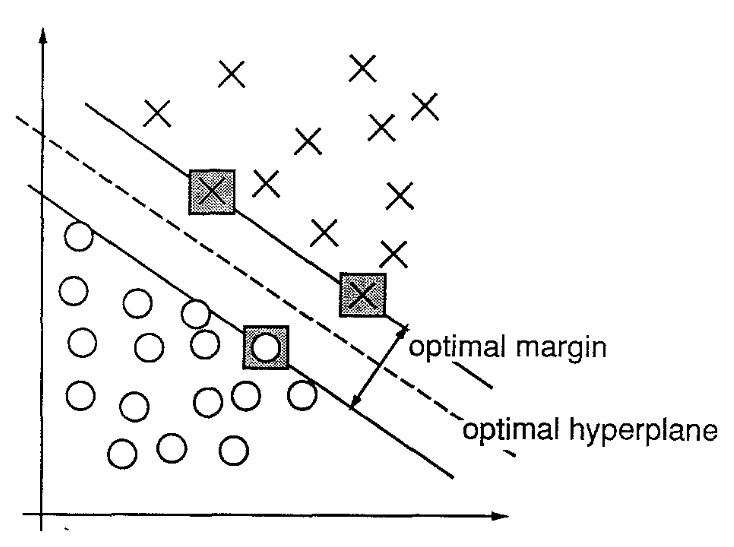
\includegraphics[width=0.6\linewidth]{./assets/images/svm-graph}
    \center\footnotesize{Fonte: \cite{Vapnik-SVM}}
    \label{fig:svm-graph}
\end{figure}

Além desta análise também são utilizadas comparações de palavras dentro de um contexto, através do uso de \textit{clusters} de palavras, que facilita a identificação de classes nos cabeçalhos analisados. Han \cite{Han-SVM} utiliza em suas análises \textit{clusters} com palavras comuns, compostos por:

\begin{itemize}
    \item Dicionário online padrão em sistemas Linux;
    \item 8.441 nomes e 19.613 sobrenomes;
    \item Sobrenomes chineses;
    \item Nomes dos estados dos Estados Unidos e das províncias canadenses;
    \item Nomes das cidades dos Estados Unidos;
    \item Nome dos países do mundo, de acordo com World Fact Book\footnote{Disponível em \url{https://www.cia.gov/library/publications/the-world-factbook/index.html}};
    \item Nome dos meses e suas respectivas abreviações.
\end{itemize}

Para cada uma das classes analisadas são feitas correlações com o tipo de dado esperado, que permite extrair, por exemplo, endereços de e-mail com base em expressões regulares utilizadas em linguagens de programação.

\emph{Support Vector Machines} é uma técnica conhecida principalmente por sua boa performance e habilidade para com grandes quantidades de dados, sendo por isso considerada uma boa solução para problemas de classificação. Por essa característica, sua principal funcionalidade é baseada na comparação entre um conjunto de opções, identificando as semelhanças e permitindo classificações. Por isso, Han \cite{Han-SVM} decidiu utilizar este mesmo conceito na extração de dados, confrontando e comparando classes de metadados, para posterior identificação e diferenciação.

Han também encontrou alguns desafios na diferenciação de campos, como é o caso dos múltiplos autores. Em alguns casos a diferenciação de autores, que fazem parte do mesmo campo, poderia estar em linhas ou grupos diferentes. Para isso foram utilizados alguns elementos para representar a separação dos nomes (\textit{chunks}), como pontuações e a presença da palavra ``and''. Desta forma, os autores eram extraídos seguindo este padrão estipulado.

O resultado obtido pela utilização de SVM como técnica de extração de metadados foi bem relevante. O autor realizou uma comparação com a aplicação da técnica de \emph{Hidden Markov Models} (HMM) - detalhada na \autoref{sssec:hmm} - onde a SVM se mostrou mais eficaz na extração para algumas classes específicas, como é o caso dos títulos, autores e endereços, por exemplo. Para outras classes a utilização da técnica de HMM ainda demonstrou ser mais eficiente na extração de metadados.

\subsubsection{Hidden Markov Models (HMM)}
\label{sssec:hmm}

A teoria básica de Markov foi conhecida próximo dos anos 80 por engenheiros e matemáticos, com grande aplicação inicialmente em processamento da fala, mas com vasta amplitude em outras áreas onde a descoberta de padrões pode ser aplicada \cite{Rabiner-HMM}.

O processo é baseado na identificação de modelos observáveis que representem e caracterizem a ocorrência de símbolos, ou seja, padrões. Se um sinal é observado ele pode ser utilizado para futuras referências, de acordo com o padrão estipulado. 

Um exemplo prático citado por Rabiner e Juang \cite{Rabiner-HMM} é o caso de uso do jogo ``Cara e Coroa''. Toma-se um observador em um quarto fechado com uma cortina, isolando totalmente qualquer outro cômodo. Este observador não consegue ver nada que acontece do outro lado, onde está presente uma outra pessoa jogando uma moeda pra cima, relatando sempre o resultado obtido (cara ou coroa). Neste caso o problema é construir um modelo Hidden Markov Model (HMM) para explicar ao observador a sequência dos resultados obtidos. 

Neste exemplo, o primeiro caso é baseado tanto no estado de cada resultado (cara ou coroa) e em probabilidades matemáticas de ocorrências destes estados, neste caso, 0.5 (50\%), ou seja, dois estados totalizando 100\%. Assim desenha-se modelos onde os estados são representados com base nas inúmeras possibilidades existentes, levando inclusive em consideração a sequência dos últimos acontecimentos. Outra possibilidade seria a existência de duas moedas, o que daria ainda dois estados existentes, mas não em função da probabilidade de sair cara ou coroa, mas sim por serem consideradas duas moedas ``justas'', o que daria também uma probabilidade de 0.5 para cada.

Neste último exemplo o grande detalhe do modelo é que este é oculto (\textit{hidden}). Isso se deve ao fato de os dois estados, representados pelas duas moedas, serem totalmente independentes, o que não permite identificar qual moeda é a ``justa'' e então informar ao observador o resultado daquela rodada.

Por esta alteração de resultados e probabilidades, o fator decisivo na criação de cada modelo é a definição do número de estados que ele terá. Além disso, outro ponto que determina o sucesso do método é a utilização de um resultado anterior - os \textit{training datasets} -, ou seja, uma memória, um conjunto de informações pré-identificadas que permite ainda à associação dos estados e ocorrência dos símbolos \cite{Rabiner-HMM}.

Um HMM pode ser formado por um conjunto de elementos, compondo toda a teoria e a aplicação dos algoritmos dentro do processo:

\begin{enumerate}
    \item Um número \texttt{N} de estados, onde \texttt{N} é um inteiro finito;
    \item Um intervalo temporal \texttt{t}, que determina a entrada em um novo estado, através de uma transição de probabilidade entre eles, levando em consideração sempre o estado anterior;
    \item Após cada transição o observador registra um \texttt{símbolo} de acordo com a distribuição de probabilidade, que por sua vez depende do estado atual do modelo.
\end{enumerate}

A utilização dos resultados passados - \textit{training datasets} - é muito importante para uma boa definição de um HMM, visto que permite adaptar os parâmetros do modelo para aquele conjunto de dados passados, que por sua vez fazem parte de um padrão já identificado e treinado.

Seguindo este padrão o HMM pode ser utilizado, por exemplo, para reconhecimento de palavras isoladas que, juntamente com a utilização de um vocabulário previamente selecionado, permite a criação de modelos de reconhecimento. Cada palavra deste vocabulário seria um modelo HMM, permitindo que a palavra escolhida fosse a pertencente ao modelo com maior probabilidade encontrada.

Já no âmbito da extração da informação, o HMM pode ser aplicado conforme é apresentado por Seymore et al. \cite{Seymore-HMM-IE}, onde um modelo construído manualmente contendo múltiplos estados por campos (título, autor, etc), pode ser mais eficiente do que um modelo com somente um estado por campo. 

\begin{figure}[h!]
    \centering
    \caption{Exemplo de modelo HMM, onde ``X'' são os estados, ``Y'' as observações possíveis, ``A'' as probabilidades de mudança de estado e ``B'' as saídas destas probabilidades.}
    \label{fig:hmm-states}
    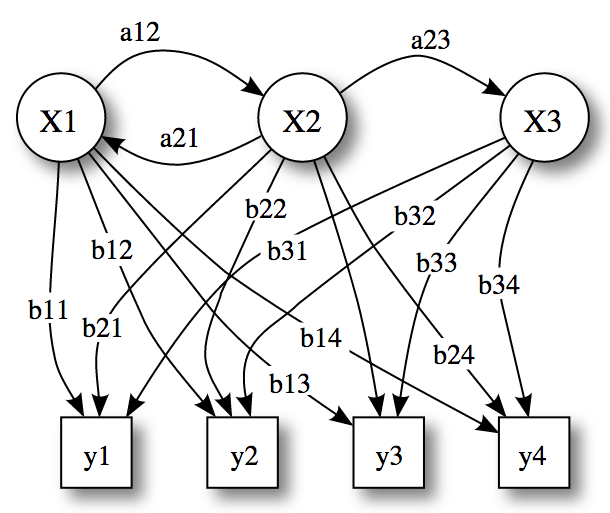
\includegraphics[width=0.7\linewidth]{./assets/images/hmm-states}
    \center\footnotesize{Fonte: Wikipedia / Hidden Markov Model \url{http://goo.gl/pI3XUU}}
\end{figure}

Um dos pontos positivos deste modelo é que, por ser baseado em estatística, ele é muito bem empregado em problemas de linguagem natural, aliando os resultados positivos à excelente performance computacional. Como desvantagem desta técnica podemos citar o fato de, por ser baseada em estatística matemática, uma grande quantidade prévia de dados deve ser utilizada - a título de treino - para se obter padrões significativos para então ser aplicados de maneira final na criação dos modelos.

Deste modo, para extração dos metadados, o HMM pode ser utilizado aplicando-se um marcador (\textit{label}) em cada palavra do cabeçalho de um documento (artigo científico), relacionando cada palavra a uma classe, como título, autor, etc. Assim, pode-se criar um modelo com \texttt{N} estados, onde cada estado corresponde a uma classe que se deseja extrair - por exemplo, o título do documento. Porém, no caso da existência de sequências ocultas (\textit{hidden sequences}) - o que alteraria a seleção do estado seguinte - a utilização de vários estados para cada classe traria resultados melhores \cite{Seymore-HMM-IE}.

% begin Seymore-HMM-IE

Para isso seria necessário entender melhor a estrutura do modelo de acordo com os dados de treino (\textit{training datasets}), utilizando-se então de múltiplos estados para cada classe, o que traria resultados melhores. Deste modo, este \textit{training dataset} permitiria a construção de um modelo chamado \textit{maximally-specific model}. Neste modelo, cada palavra do \textit{training dataset} seria associada com seu próprio estado, com transição para o estado correspondente à palavra seguinte \cite{Seymore-HMM-IE}.

Este modelo, segundo os autores, poderia ser usado como ponto de partida de uma variedade de técnicas para junção de estados (\textit{state merging techniques}). Desta forma os autores propõem duas formas de junção de estados que permitam a construção deste \textit{maximally-specific model}:

\begin{enumerate}

\item \textit{\textbf{Neighbor-merging:}} combina todos os estados que compartilham transições e possuem o mesmo nome de classe. Por exemplo, estados correspondentes ao título seriam reunidos em apenas um estado. Assim, vários estados vizinhos com os mesmos nomes de classes seriam transformados em apenas um.

\item \textit{\textbf{V-merging:}} combina quaisquer dois estados que possuem o mesmo nome de classe e compartilham transições ``de'' ou ``para'' um estado comum. Desde modo, ao invés de começar no estado inicial e decidir para qual estado correspondente ao título será feita a transição, esta técnica juntaria os estados ``filhos'' em um único estado, de maneira que somente uma transição do estado inicial para o estado de título poderia existir. Desta forma, esta técnica poderia ser utilizada como modelo direto para a extração de dados, podendo também criar novas combinações de estados, implicando em uma melhoria deste modelo.

\end{enumerate}

Como o objetivo de Seymore et al. é extrair informações relevantes de cabeçalhos de artigos de Ciência da Computação, a área de cobertura nestes documentos limita-se até o início da introdução, ou ao final da primeira página, o que ocorrer primeiro.

O resumo (\textit{abstract}) é extraído facilmente com a utilização de expressão regular (\autoref{sssec:regular-expressions}). Algumas classes de palavras especiais são identificadas também através de expressão regular e então são transformadas em \textit{tags} ou \textit{tokens}, como \texttt{<EMAIL>} ou \texttt{<YEAR\_NUMBER>}, por exemplo. Em todos estes casos, todos os acentos e informações de novas linhas (\texttt{\textbackslash{n}}) são removidos do texto.

Os resultados apontam como muito positiva a utilização de HMM para a extração de dados em cabeçalhos de artigos científicos. A precisão encontrada no experimento foi de 92,9\% para todas as classes do cabeçalho e, mais especificamente, 97,2\% para a extração dos autores. Também como resultado pode-se afirmar que modelos HMM com mais de um estado por classe são mais eficientes do que modelos que utilizam apenas um estado para cada classe analisada \cite{Seymore-HMM-IE}.

% end Seymore-HMM-IE

Uma outra utilização de HMM na extração de informação é descrita por \cite{Zhang-HMM-IE}, onde é realizado um experimento de extração de informação utilizando um conjunto de dados semi-estruturados, em formato HTML, contendo informações sobre restaurantes da cidade de Los Angeles.

Neste caso são estipulados quatro estados para o modelo: \textit{Background}, \textit{Prefix}, \textit{Suffix} e \textit{Target}. O \textit{Target} é o estado responsável pela emissão do símbolo - chamado pelo autor de \textit{token} - para o ``campo-alvo''. O \textit{Prefix} e \textit{Suffix} são estados que emitem símbolos que aparecem respectivamente antes e depois desse campo-alvo. Todos os demais símbolos são emitidos no estado \textit{Background}. A relação entre os estados pode ser visualizada na \autoref{fig:zhang-hmm-ie}.

\begin{figure}[h!]
    \centering
    \caption{Estados utilizados por \cite{Zhang-HMM-IE} em seu modelo HMM.}
    \label{fig:zhang-hmm-ie}
    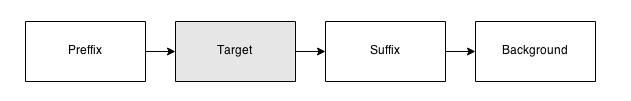
\includegraphics[width=0.8\linewidth]{./assets/images/zhang-hmm-ie}
    \center\footnotesize{Fonte: O próprio autor.}
\end{figure}

Os seguintes campos deveriam ser extraídos das informações dos restaurantes: \textit{restaurant name} (nome do restaurante), \textit{telephone number} (número de telefone), \textit{hours} (horas) e \textit{cuisine} (tipo de comida servida, como italiana, alemã, etc). Segundo Zhang \cite{Zhang-HMM-IE} os campos \textit{restaurant name} e \textit{telephone number} deveriam ser mais fáceis de serem obtidos, visto que o nome do restaurante geralmente se encontra em destaque, com alguma diferenciação visual. Já o telefone possui um formato numérico, que permite mais facilmente uma identificação de um padrão. O campo \textit{hours} também não seria complicado, embora se tenha uma variedade muito grande na representação desta informação. Já o campo \textit{cousine} foi mais difícil de ser extraído, visto a diversidade que existe na forma de um restaurante especificar e/ou representar sua cozinha, tanto na utilização de palavras diferentes quanto na própria identificação do estilo do restaurante por si só.

Como resultados esperados, os campos \textit{restaurant name} e \textit{telephone number} obtiveram muito êxito em sua extração, com resultados realmente consideráveis. Já os campos \textit{hours} e \textit{cousine} não tiveram resultados muito satisfatórios, o que pode ser explicado em função da característica dos HMMs de utilizar como modelo resultados de aprendizados anteriores, os \textit{training datasets}. Como nestes dois campos há uma grande possibilidade de representação, os resultados não foram tão eficazes, o que poderia ser resolvido com uma alteração no modelo HMM que permitisse que as palavras identificadas como sendo do campo \textit{cousine} fossem capturadas de maneira mais proveitosa, que estão, neste modelo sugerido, isoladas no estado \textit{Background}.

Em função dos resultados obtidos, pode-se considerar a performance do HMM na extração de informação como positiva, visto as possibilidades de variação do modelo, que permite um resultado mais preciso e próximo dos objetivos reais \cite{Zhang-HMM-IE}. Além disso, a utilização de resultados passados garante um aprendizado importante para que o modelo seja estabelecido, o que garante ainda mais um ganho de eficiência na aplicação desta técnica.

Além da utilização de HMM de forma natural, algumas variações de seu algoritmo são também citadas na literatura, como é o caso dos MEMMs (\textit{Maximum Entropy Markov Models}) \cite{maximum-entropy}. Nos MEMMs cada estado possui um modelo exponencial que utiliza as características de observação como entrada de dados (\textit{input}) \cite{Lafferty-CRF}. Estes modelos são baseados na técnica de HMM, se diferenciando na maneira como os estados se relacionam, bem como a relação entre suas transições, levando a citações independentes por alguns autores, porém, com herança conceitual dos modelos HMM.

\subsubsection{Word Clustering}
\label{sssec:word-clustering}

Técnicas de classificação de texto geralmente utilizam palavras extraídas como a principal fonte de recursos para a representação. Por outro lado, os \textit{clusters} de palavras tem sido uma proposta eficaz para a redução da dimensionalidade e da dispersão, melhorando assim a performance desta classificação \cite{Han-Giles-WC}.

O conceito de \textit{clusters} compreende um conjunto de palavras que formam um banco de dados de domínio (\textit{domain database}), que é aliado a um conjunto de propriedades ortográficas de palavras dentro do contexto específico. A utilização destes \textit{clusters}, juntamente com outras técnicas, tem mostrado um ganho de 6,6\% na performance de classificação de elementos de um cabeçalho de artigo científico, e ainda 8,4\% de ganho de performance para a extração das referências destes documentos \cite{Han-Giles-WC}.

A utilização destes grupos de palavras demonstra uma relação entre textos semelhantes dentro de um determinado contexto, permitindo que a extração dos metadados ocorra de maneira natural, com resultados mais eficazes.

Sendo assim, Han et al. apresentaram uma ideia de um \textit{cluster} de palavras para promover a extração de metadados de artigos científicos da área de Ciência da Computação, indo de maneira contrária às propostas mais tradicionais, que se baseiam, geralmente, apenas na ocorrência e estatísticas de palavras isoladas dentro do texto original.

Han et al. agruparam bases de dados de domínios diversos incluindo também propriedades ortográficas de palavras, com base em um conhecimento prévio de classes específicas, como autor, título, etc. Deste modo, palavras encontradas nos documentos vão sendo comparadas com palavras deste \textit{cluster}, permitindo identificar, por grupos, características semelhantes de metadados. Para cada classe (metadado) cria-se um \textit{cluster}, com suas palavras e propriedades ortográficas específicas.

Como exemplo, a palavra ``Mary'' faz parte do \textit{cluster} de ``nomes''. Portanto, existe uma probabilidade maior de ela, juntamente com seu grupo de palavras ao redor, fazer parte da classe ``autor'', por exemplo. Esta lógica é apresentada também para outras classes, como ``e-mail'' por exemplo, que pode ser identificado com a presença do caractere ``@'', levando à utilização de expressões regulares para encontrar padrões de ocorrências (\autoref{sssec:regular-expressions}).

\begin{figure}[h!]
    \centering
    \caption{\emph{Workflow} da extração de metadados usando \textit{cluster} de palavras.}
    \label{fig:workflow-rule-based}
    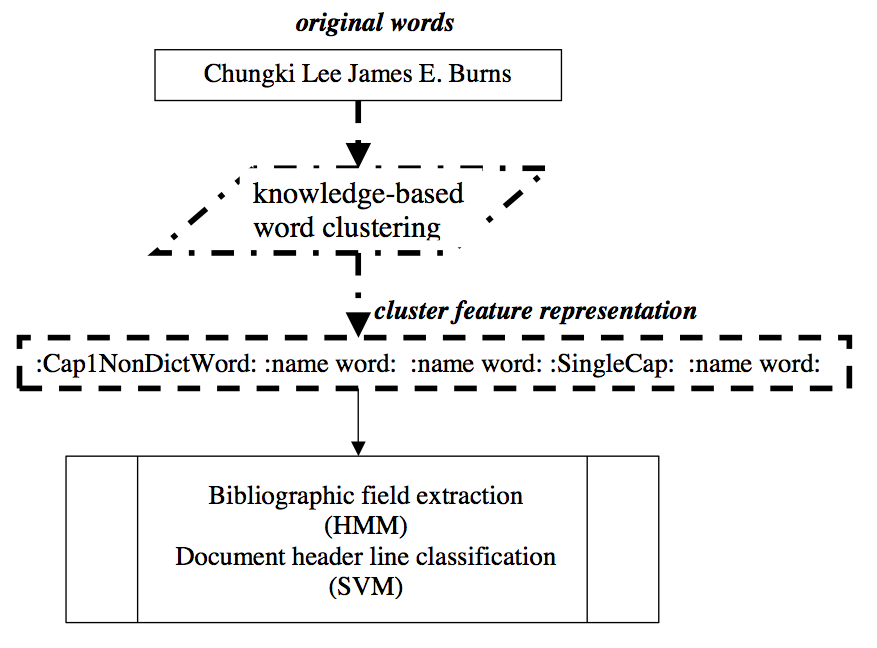
\includegraphics[width=0.7\linewidth]{./assets/images/workflow-rule-based}
    \center\footnotesize{Fonte: \cite{Han-Giles-WC}}
\end{figure}

A utilização de \textit{word clustering} possui um custo computacional muito baixo, o que pode ser considerado uma vantagem sobre demais técnicas computacionais \cite{Han-Giles-WC}.

Han et al. ainda utilizam da técnica de SVM (\autoref{sssec:svm}) para classificação de linhas de um cabeçalho de um documento, tanto em função dos bons resultados obtidos, quanto também pela boa performance apresentada. Deste modo, cada linha obtida se transforma em um vetor de palavras, que é comparado com seu respectivo \textit{cluster}, melhorando os resultados de classificação, unindo as duas técnicas em prol do mesmo objetivo.

A técnica de \textit{Word Clustering} se resume em 3 (três) etapas. A primeira compreende a construção das bases de dados, como referenciado por Han \cite{Han-SVM}, onde foram utilizadas também bases externas - nomes de estados americanos, países, cidades, nomes de dicionários, nomes de pessoas, códigos postais, etc -, unindo também bases construídas dentro de um domínio específico, como palavras pertencentes a uma classe específica.

A segunda etapa é chamada de \textit{Cluster Design}. Nesta etapa os \textit{clusters} são arquitetados, contemplando também propriedades ortográficas das palavras, formando então o dicionário com base nas características apresentadas.

Já a terceira etapa é chamada de \textit{Rule Design}, que consiste na combinação de palavras em diferentes domínios, nas suas verificações ortográficas e na classificação delas em seu \textit{cluster} correto. Por exemplo, nomes devem começar com a primeira letra maiúscula para então serem classificadas como pertencentes ao \textit{cluster} ``nomes''.

Além disso, foi observada também a presença de certas palavras que faziam parte de diversos \textit{clusters} ao mesmo tempo, o que permitiu que elas fossem classificadas em seu próprio grupo de palavras, tornando-se então independentes.

A representação através de \textit{clusters}, utilizada por Han et al. \cite{Han-Giles-WC}, conseguiu reduzir um texto original de 11.223 palavras em um \textit{cluster} de 588 elementos, permitindo ainda que ele fosse distribuído entre classes distintas, o que tornou o processo muito menos trabalhoso, porém mais eficaz.

Como resultado, a utilização desta técnica de clusterização permitiu um ganho considerável de performance, além de contribuir para uma precisão maior dos resultados, visto que são apresentados dentro de um domínio específico, perfazendo um contexto mais definido e com resultados mais garantidos.

Por outro lado a utilização desta técnica possui uma falha na semântica dos dados. No momento da classificação de classes, na separação e criação dos \textit{clusters}, por exemplo, um dígito ou conjunto deles é substituído pela identificação \texttt{:number:}. Isso faz com que ele se torne apenas um número qualquer, sem uma semântica específica, ou seja, pode ser tanto uma referência a alguma página do documento ou até mesmo um mês ou ano, por exemplo.


\subsubsection{Conditional Random Fields (CRFs)}
\label{sssec:crf}

% Falar sobre CRFs 

CRFs é um framework proposto por Lafferty et al. \cite{Lafferty-CRF} criado para construir modelos probabilísticos e dados marcados em sequência (\textit{label sequence data}), geralmente utilizados no reconhecimento de padrões e aprendizado de máquina (\textit{machine learning}).

Esta técnica oferece algumas vantagens se comparada com técnicas mais tradicionais, como HMM (\autoref{sssec:hmm}), se destacando a habilidade de diminuir pressupostos independentes feitos nestes modelos \cite{Lafferty-CRF}.

Modelos baseados em HMM possuem uma fraqueza, que é o problema denominado \textit{bias problem}. As transições de um estado somente competem entre elas, e não com todas as transições presentes no modelo. Elas são feitas com base probabilística de acordo com o estado inicial e a sequência de observação (\textit{observation sequence}) \cite{Lafferty-CRF}.

Desta forma, devido ao \textit{bias problem}, em um caso extremo, um estado que tiver como opção de transição somente um outro estado, pode simplesmente ignorar a sequência de observação, o que traria efeitos contrários aos objetivos do processo inicial.

Lafferty et al. realizam comparações funcionais e práticas entre CRFs, HMM e MEMM (\textit{Maximum Entropy Markov Models}), uma variação da técnica de HMM, detalhada na \autoref{sssec:hmm}. A importante diferença entre CRFs e MEMMs é que MEMM utiliza modelos exponenciais como probabilidade de ocorrência de um próximo estado, enquanto a técnica de CRF possui um modelo exponencial único para toda a sequência de \textit{labels}, com base na sequência de observação. Segundo Lafferty et al. \cite{Lafferty-CRF} pode-se pensar na CRF como um modelo de estado finito sem normalização das probabilidades de transição.

Uma das vantagens de se utilizar CRFs sobre HMM é que ela absorve boa parte de suas qualidades, mas com a particularidade de resolver o \textit{bias problem}. Outra grande vantagem sobre HMMs e MEMMs é que a CRF possui resultados melhores quando a distribuição dos dados possui grande dependência do modelo, o que geralmente ocorre em casos mais práticos.

Um exemplo para entender o \textit{bias problem} foi também apresentado por Lafferty et al. \cite{Lafferty-CRF}. Ele propõe um modelo cujo objetivo é distinguir duas palavras: \texttt{rib} e \texttt{rob}, tendo como sequência de observação as letras \texttt{r i b}. O problema é identificado quando uma das duas palavras é mais comum no \textit{training set}, o que acarreta nas transições do estado inicial preferirem suas transições correspondentes, o que acaba sempre na vitória da palavra relacionada àquele estado.

Visando a comprovação e reconhecimento da eficiência da técnica de CRF na extração de informação foram aplicados dois tipos de experimentos:

\begin{enumerate}
    \item Verificação direta do \textit{bias problem};
    \item Geração de dados utilizando HMM aleatórios.
\end{enumerate}

Os resultados apontam que HMMs superam MEMMs em virtude do \textit{bias problem}. Por sua vez os CRFs superam os HMMs, sendo então considerada a melhor técnica para ser empregada com base no \textit{training set} utilizado \cite{Lafferty-CRF}. Outro ganho apresentado pode ser verificado ao agregar algumas características ortográficas à utilização de CRFs, aumentando o poder destes modelos condicionais.

De modo geral as CRFs utilizam a mesma lógica que modelos baseados em Markov (HMMs e MEMMs), se diferenciando nos aspectos probabilísticos para com as transições entre os estados, acarretando em resultados comparativamente melhores. Por corresponder a uma ``máquina'' de estado finito, a técnica é muito aplicável para funções de classificação sequencial, o que permite que seja treinada para se obter os melhores resultados probabilísticos \cite{Peng-CRF-IE}. Nas CRFs as transições de estado são também representadas como \emph{features} por alguns autores.

%Esta técnica é comparada e quase sempre utilizada juntamente com a HMM (Hidden Markov Models), de maneira a possuir algumas vantagens sobre esta última, como a habilidade de relacionar pressupostos independentes nos modelos, ou seja, relacionar observações e/ou interpretações.

Uma outra vantagem da técnica de CRFs - assim como dos modelos \emph{maximum entropy} - é que eles permitem o uso de características arbitrárias nos dados de entrada. As CRFs são utilizadas também em marcação e classificação de dados sequenciais, como linguagem natural, sequências biológicas (como os genes) ou estados computacionais.

% Falar sobre o uso de CRFs na extração de informação

Sua aplicação na extração de metadados foi apresentada por Peng et al. \cite{Peng-CRF-IE}, como uma maneira eficaz de extrair metadados em cabeçalhos e referências de artigos científicos. Deste modo, através da identificação destes padrões sequenciais pode-se determinar os tipos de dados existentes e então identificá-los, seguindo uma lógica/ordem pré-determinada.

Peng et al. apresentam resultados desta extração utilizando Conditional Random Fields (CRF) e aponta também algumas questões acerca da utilização testa técnica para este tipo de atividade. Os autores comparam as CRFs com técnicas de HMM (\autoref{sssec:hmm}) e SVM (\autoref{sssec:svm}), mencionando que a forma de trabalhar com CRF aponta parte das vantagens destas duas técnicas, destacando a junção entre as sequências e características dependentes, mas ao mesmo tempo arbitrárias. Ainda assim, segundo os autores, a utilização de CRFs para a tarefa de extração de metadados - ao se comparar com as demais técnicas de SVM e HMM - possui melhoras significativas.

Os autores definem quatro diferentes transições de estado para diferentes classes, em ordem diferente das técnicas derivadas de Markov (HMM):

\begin{enumerate}
    \item \emph{\textbf{First-order:}} os dados de entrada são examinados no contexto de somente um estado;
    \item \emph{\textbf{First-order + transitions:}} são adicionados alguns parâmetros correspondentes às transições;
    \item \emph{\textbf{Second-order:}} as entradas são examinadas no contexto dos estados atual e anterior;
    \item \emph{\textbf{Third-order:}} os dados de entrada são examinados no contexto do estado atual e de dois estados anteriores.
\end{enumerate}

Para a extração destes dados Peng et al. \cite{Peng-CRF-IE} também consideram como sendo o cabeçalho de um artigo como sendo a parte inicial do documento até a introdução, ou somente a primeira página, o que ocorrer primeiro. Além disso, os autores consideram como os campos a serem analisados os mesmos 15 (quinze) que foram definidos anteriormente por Seymore et al. \cite{Seymore-HMM-IE}.

Para extração dos metadados dos cabeçalhos foi utilizado um \emph{dataset} \cite{Peng-CRF-IE} com 935 (novecentos e trinta e cinco) documentos. Destes, 500 (quinhentos) foram utilizados para compor o \emph{training set} e os outros 435 (quatrocentos e trinta e cinco) para fins de teste, unicamente. Já do \emph{dataset} utilizado para extração das referências foram analisados 500 (quinhentos) documentos, dos quais 350 (trezentos e cinquenta) foram utilizados para o \emph{training set} e os demais 150 (cento e cinquenta) também para testes.

Para fins de resultados comparativos foram utilizadas três métricas:

\begin{enumerate}

    \item \emph{\textbf{Overall word accuracy:}} é uma métrica que utiliza a porcentagem de palavras das quais os nomes (\emph{labels}) previstos são exatamente seus valores reais. Esta métrica favorece aqueles campos que possuem muitas palavras, como, por exemplo, a introdução (\emph{abstract});

    \item \emph{\textbf{Average F-measure (F1):}} esta métrica se baseia na exatidão das ocorrências, considerando tanto a precisão quanto a memória de todos os campos (\emph{fields}). Esta métrica favorece campos com poucas palavras, visto sua característica mais importante, de focar na exatidão dos resultados.
    
    \item \emph{\textbf{Whole instance accuracy:}} nesta métrica uma ``instância'' é considerada como sendo todo um cabeçalho ou referência, de maneira integral. Desta forma esta métrica utiliza-se da porcentagem de instâncias das quais cada palavra é corretamente associada.

\end{enumerate}

Conforme pode-se observar na \autoref{tab:crf-results-headers} e \autoref{tab:crf-results-references} a utilização de CRFs para extração de metadados - tanto de cabeçalhos como de referências - teve resultados melhores do que a utilização de HMM (\autoref{sssec:hmm}), aumentando a performance em praticamente todos os campos, chegando a uma precisão de 98,3\% (\emph{overall accuracy}).

Pode-se observar também que a utilização de modelos HMM para precisão de palavras (campos com poucas palavras, onde a precisão é muito mais importante) é, de modo geral, pior do que quando utiliza-se de SVMs (coluna F1 da \autoref{tab:crf-results-headers}). Por outro lado, no campo \emph{abstract} HHM possui performance bem melhor que quando utilizado SVM (98\% contra 93,8\%).

\begin{table}[h!]
    \caption{Resultados de extração para CRFs após análise do \emph{dataset} com cabeçalhos \cite{Peng-CRF-IE}.}
    \begin{center}
        \begin{tabular}{|c|c|c|c|c|c|c|} \hline             
             & \multicolumn{2}{c|}{HMM} & \multicolumn{2}{c|}{CRF} & \multicolumn{2}{c|}{SVM} \\  \hline 
            Overall acc. & \multicolumn{2}{c|}{93.1\%} & \multicolumn{2}{c|}{\textbf{98.3\%}} & \multicolumn{2}{c|}{92.9\%} \\ \hline
            Instance acc. & \multicolumn{2}{c|}{4.13\%} & \multicolumn{2}{c|}{\textbf{73.3\%}} & \multicolumn{2}{c|}{-} \\ \hline \hline
             & acc. & F1 & acc. & F1 & acc. & F1 \\ \hline
            Title & 98.2 & 82.2 & 99.7 & \textbf{97.1} & 98.9 & 96.5 \\ \hline
            Author & 98.7 & 81.0 & 99.8 & \textbf{97.5} & 99.3 & 97.2 \\ \hline
            Affiliation & 98.3 & 85.1 & 99.7 & \textbf{97.0} & 98.1 & 93.8 \\ \hline
            Address & 99.1 & 84.8 & 99.7 & \textbf{95.8} & 99.1 & 94.7 \\ \hline
            Note & 97.8 & 81.4 & 98.8 & \textbf{91.2} & 95.5 & 81.6 \\ \hline
            Email & 99.9 & 92.5 & 99.9 & \textbf{95.3} & 99.6 & 91.7 \\ \hline
            Date & 99.8 & 80.6 & 99.9 & \textbf{95.0} & 99.7 & 90.2 \\ \hline
            Abstract & 97.1 & 98.0 & 99.6 & \textbf{99.7} & 97.5 & 93.8 \\ \hline
            Phone & 99.8 & 53.8 & 99.9 & \textbf{97.9} & 99.9 & 92.4 \\ \hline
            Keyword & 98.7 & 40.6 & 99.7 & \textbf{88.8} & 99.2 & 88.5 \\ \hline
            Web & 99.9 & 68.6 & 99.9 & \textbf{94.1} & 99.9 & 92.4 \\ \hline
            Degree & 99.5 & 68.8 & 99.8 & \textbf{84.9} & 99.5 & 70.1 \\ \hline
            Pubnum & 99.8 & 64.2 & 99.9 & 86.6 & 99.9 & \textbf{89.2} \\ \hline
            \hline
            Average F1 & & 75.6 & & \textbf{93.9} & & 89.7 \\ \hline
        \end{tabular}
    \end{center}
    \label{tab:crf-results-headers}
\end{table}

\begin{table}[h!]
    \caption{Resultados de extração para CRFs após análise do \emph{dataset} com referências \cite{Peng-CRF-IE}.}
    \begin{center}
        \begin{tabular}{|c|c|c|c|c|} \hline             
             & \multicolumn{2}{c|}{HMM} & \multicolumn{2}{c|}{CRF} \\  \hline 
            Overall acc. & \multicolumn{2}{c|}{85.1\%} & \multicolumn{2}{c|}{\textbf{95.37\%}} \\ \hline 
            Instance acc. & \multicolumn{2}{c|}{10\%} & \multicolumn{2}{c|}{\textbf{77.33\%}} \\ \hline \hline
             & acc. & F1 & acc. & F1 \\ \hline 
            Author & 96.8 & 92.7 & 99.9 & \textbf{99.4} \\ \hline 
            Booktitle & 94.4 & 0.85 & 97.7 & \textbf{93.7} \\ \hline 
            Date & 99.7 & 96.9 & 99.8 & \textbf{98.9} \\ \hline 
            Editor & 98.9 & 70.8 & 99.5 & \textbf{87.7} \\ \hline 
            Institution & 98.5 & 72.3 & 99.7 & \textbf{94.0} \\ \hline 
            Journal & 96.6 & 67.7 & 99.1 & \textbf{91.3} \\ \hline 
            Location & 99.1 & 81.8 & 99.3 & \textbf{87.2} \\ \hline 
            Note & 99.2 & 50.9 & 99.7 & \textbf{80.8} \\ \hline
            Pages & 98.1 & 72.9 & 99.9 & \textbf{98.6} \\ \hline
            Publisher & 99.4 & \textbf{79.2} & 99.4 & 76.1 \\ \hline
            Tech & 98.8 & 74.9 & 99.4 & \textbf{86.7} \\ \hline
            Title & 92.2 & 87.2 & 98.9 & \textbf{98.3} \\ \hline
            Volume & 98.6 & 75.8 & 99.9 & \textbf{97.8} \\ \hline
            \hline
            Average F1 & & 77.6\% & & \textbf{91.5\%} \\
            \hline
        \end{tabular}
    \end{center}
    \label{tab:crf-results-references}
\end{table}

Com base nos resultados apresentados pode-se considerar que o trabalho de Peng \cite{Peng-CRF-IE} contribuiu para o estado da arte, melhorando a performance na extração de metadados em artigos científicos. Assim, a utilização de CRFs mostra-se muito eficaz por reduzir consideravelmente os erros encontrados, aumentando o sucesso da aplicação desta técnica neste contexto.

\section{Trabalhos Correlatos}
\label{sec:revision}

% Falar aqui sobre os estudos de comparações de Granitizer

Técnicas de \emph{machine learning} não são novas, porém suas aplicações são inúmeras. Estas técnicas inicialmente eram utilizadas apenas para classificação de palavras e processamento de linguagem natural, mas foram sendo utilizadas em diversas outras áreas resolvendo problemas distintos e inovando em soluções, como é o caso da extração de informação.

O aperfeiçoamento da aplicação destas técnicas para a área de extração de informação acarretou em um resultado muito positivo, melhorando a precisão dos resultados obtidos. Assim, algoritmos foram/são alterados e otimizados visando obter maiores performances e resultados cada vez melhores.

Pode-se perceber que cada técnica de classificação e/ou extração de informação possui suas particularidades e características diferentes. Assim, é possível notar, em grande parte, que algumas possuem uma melhor aplicação para extração de determinado campo, ou conjunto deles. Pequenas modificações são necessárias para que todo o contexto de um artigo científico seja mapeado com sucesso, sendo às vezes necessária a utilização de diversas técnicas em um único projeto.

Para isso, diversas comparações entre técnicas foram feitas. Algumas - inclusive já mencionadas ao longo deste capítulo - foram feitas quando do surgimento de uma nova técnica, onde esta era comparada com técnicas anteriores. Porém, este tipo de comparação torna-se tendenciosa, visto que os campos analisados, bem como os \emph{datasets} utilizados, tendenciam para resultados positivos da nova técnica apresentada. Além disso, geralmente os \emph{datasets} utilizados são focados em documentos da área de Ciência da Computação, e tendem a seguir um padrão visual já estipulado pelos grandes eventos da área.

Em função deste problema alguns autores realizam comparações de técnicas, isoladamente ou com utilização de ferramentas, para analisar um grupo de documentos reais, objetivando um resultado mais próximo da realidade e, consequentemente, mais passível de erros. Estas comparações são relevantes para o Estado da Arte deste trabalho.

Granitzer et al. \cite{Granitzer-2012-LayoutBased} comparam o uso de Conditional Random Fields (\autoref{sssec:crf}) e Support Vector Machines (\autoref{sssec:svm}) na extração de metadados em artigos científicos. Para isso são utilizados \emph{datasets} multidisciplinares, como \emph{Mendeley} e \emph{e-Prints}, que fazem parte de um grupo social de \emph{datasets}, permitindo uma contribuição global entre pesquisadores de diversas áreas do conhecimento.

Em virtude da existências destes repositórios a informação fica cada vez mais descentralizada e, portanto, são necessários cada vez mais mecanismos inteligentes para garantir a alta qualidade dos metadados extraídos \cite{Granitzer-2012-LayoutBased}. A combinação destes mecanismos com pós-processamento inteligente contribui para o processo, elevando a qualidade do resultado final encontrado.

% CiteSeer e Mendeley utilizam SVMs. Granitzer 2012

Visando um reconhecimento maior dos resultados obtidos, Granitzer et al. realizam comparações dos resultados com a aplicação de três ferramentas: ParsCit (\autoref{ssec:parscit}), Mendeley Desktop (\autoref{ssec:mendeley}) e sua própria ferramenta baseada em CRFs, no qual se referem como ``Layout-based CRF''.

Este trabalho \cite{Granitzer-2012-LayoutBased} é uma continuação do trabalho anteriormente realizado \cite{Granitzer-2012-Crowdsourced}, onde as ferramentas Mendeley Desktop (\autoref{ssec:mendeley}) e ParsCit (\autoref{ssec:parscit}) foram comparadas, utilizando, porém, um \emph{dataset} menor. Desta vez foi incluída a técnica de Conditional Random Fields (CRF) na comparação que, de acordo com a literatura mencionada neste trabalho, possui resultados melhores do que a utilização de Hidden Markov Models (HMMs - \autoref{sssec:hmm}).

Foram analisadas 20.672 publicações do \emph{dataset} Mendeley \cite{Granitzer-2012-LayoutBased}, abrangendo diversas áreas do conhecimento como Ciência de modo geral, Ciência da Computação, Biomedicina e Física. Já no \emph{dataset} e-Prints foram analisadas 2.452 publicações de áreas como Física, Medicina e diversas outras pertencentes ao IEEE, ligadas geralmente à área de computação.

Foi relatado que uma das etapas principais para um bom processamento e uma boa precisão é o ``pós-processamento''. A aplicação de diversas análises (inclusive matemáticas) nos resultados extraídos garante um conjunto de dados de saída muito melhor e mais acurado. Segundo Granitzer et al. \cite{Granitzer-2012-LayoutBased} estas tarefas são de responsabilidade do setor de engenharia, onde diversos detalhes devem ser observados e diversos algoritmos aplicados.

De modo geral, os resultados obtidos pelas ferramentas Mendeley e ParsCit foram considerados ruins para os grupos pertencentes à área médica \cite{Granitzer-2012-LayoutBased}. Porém, estes resultados poderiam ser melhorados com um novo treino dos dados (\emph{training set}), com aplicações específicas para aquela área do conhecimento, no caso, a medicina. Outro ponto interessante observado \cite{Granitzer-2012-LayoutBased} foi o fato de a extração dos títulos ter ocorrido mais facilmente do que a extração dos autores, variando a performance dos resultados em função da técnica utilizada.

Para os outros grupos os resultados foram bem positivos, observando uma pequena diferença entre os números obtidos com as ferramentas Mendeley e ParsCit, que foram muito superiores aos resultados da implementação CRF dos autores. Isso se deve ao fato das duas ferramentas anteriores utilizarem de pós-processamento dos dados, o que garantiu aos resultados obtidos uma precisão muito maior \cite{Granitzer-2012-LayoutBased}.

De acordo com Granitzer et al., mesmo a técnica de CRF possuindo melhores modelos de extração de informação, foi-se observado que a técnica de SVM utilizada pelo Mendeley Desktop supera a CRF no que tange extração de metadados \cite{Granitzer-2012-LayoutBased}.

A ferramenta ParsCit de modo geral não teve resultados melhores que o Mendeley Desktop \cite{Granitzer-2012-LayoutBased}. Para a área de Ciência da Computação, mais especificamente na base de dados do IEEE, ambas as ferramentas obtiveram excelentes resultados. Já na base de dados da ACM o Mendeley obteve melhores resultados do que o ParsCit \cite{Granitzer-2012-LayoutBased}.

\section{Ferramentas de Extração de Metadados}
\label{sec:environments}

Algumas ferramentas fundamentam suas funcionalidades de extração em padrões pré-definidos, identificando dados relevantes dentro de uma região específica dos artigos, o que facilita a procura e consequentemente aumenta a velocidade nos resultados finais.

Estas ferramentas geralmente permitem uma variedade muito grande de leiautes, embora nem todos já estejam previamente definidos. Geralmente suporte a novos leiautes são inseridos em novas versões ou até mesmo por contribuições das mais diversas, como é o caso dos projetos de código livre, os chamados projetos \textit{open source}.

Abaixo segue uma relação das principais ferramentas relacionados à área de extração de metadados em artigos científicos, com informações sobre sua história, funcionamento e algumas técnicas que utilizam.

\subsection{Cermine}
\label{ssec:cermine}

% CERMINE

Uma destas ferramentas é o recente Cermine \cite{cermine}, uma biblioteca \textit{open source} desenvolvida na linguagem de programação Java que permite que sejam extraídos os metadados de artigos científicos em formato digital PDF, oferecendo ainda a possibilidade de cruzamento de dados por meio de referências e títulos, permitindo assim identificar citações bem como a relevância de um determinado documento.

O Cermine ainda possui um mecanismo de aprendizagem próprio que permite que, na medida que dados forem sendo alterados, ele consiga absorver os detalhes passados e realizar mudanças em sua forma de realizar a extração. Deste modo ele permite adaptações para novos padrões de leiautes, o que permite de maneira geral que uma grande gama de modelos seja então abrangida. 

Seu grande diferencial em comparação com as demais ferramentas é que ele não somente extrai os metadados de um artigo, mas também analisa todo o seu conteúdo, incluindo citações a outros documentos, que podem ser facilmente cruzados por meio de informações como título e autor(es).

Seu mecanismo considera arquivos PDF em forma textual, sem a utilização de imagens, ou seja, não abrange documentos gerados a partir de artigos escaneados. A ferramenta considera regiões, linhas e páginas como pontos estratégicos para a extração de informações. As bases destas regiões possuem padrões que são utilizados juntamente com técnicas de SVM \cite{Han-SVM} (detalhado na \autoref{sssec:svm}). Dessa forma seu mecanismo condensa um leiaute onde as informações geralmente estão dispostas, permitindo aferir que em um determinado local do arquivo estejam o título e o nome dos autores, por exemplo. 

Com estas regiões definidas o Cermine extrai as informações com base em padrões preestabelecidos, gerando resultados para os metadados e referências encontradas. O formato de saída dos resultados é no formato XML, permitindo que possam ser compartilhados com outros sistemas por possuir uma leitura semântica e ao mesmo tempo fácil de ser interpretada pelas linguagens de programação. A \autoref{fig:cermine-workflow} demonstra como o processo de extração do Cermine funciona.

\begin{figure}[h!]
    \centering
    \caption{Cermine Extraction Workflow}
    \label{fig:cermine-workflow}
    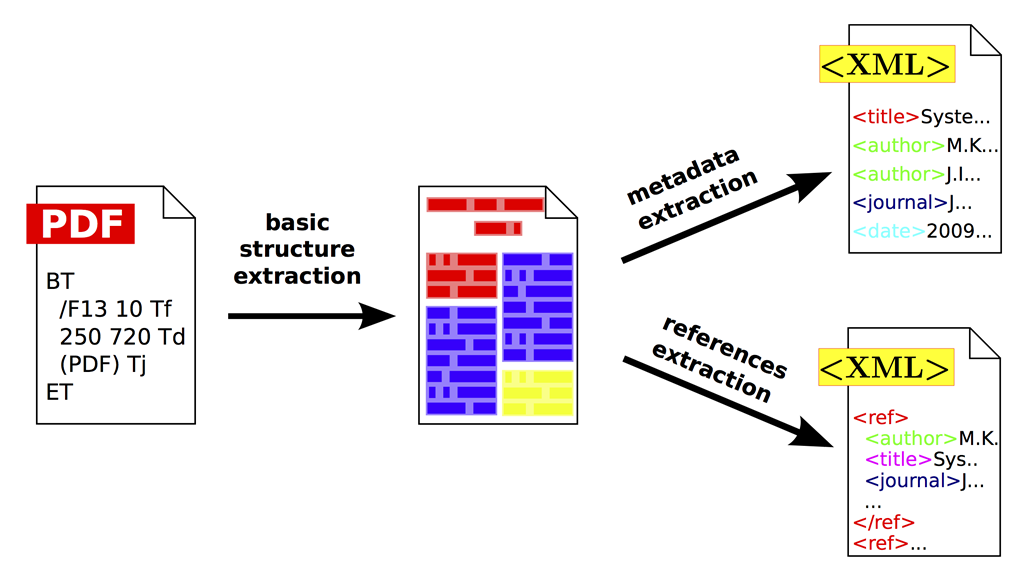
\includegraphics[width=0.7\linewidth]{./assets/images/cermine}
    \center\footnotesize{Fonte: \cite{cermine}}
\end{figure}

Após o mapeamento definido a ferramenta identifica regiões de acordo com seu conteúdo de entrada, as quais ele chama de \textit{zones}. Estas regiões são determinadas a fim de extrair suas informações mais relevantes, separando, por exemplo, a área destinada aos metadados do arquivo. O Cermine divide estas \textit{zones} da seguinte maneira:

\begin{itemize}

    \item \textbf{Metadata:} É a região mais ao alto do documento, onde obtém os metadados, que seriam o resumo, \textit{bib\_info}, tipo, título, afiliação, autores, datas, editores e palavras-chaves.

    \item \textbf{References:} Região responsável por identificar detalhes de referências que foram utilizadas no artigo, como título e autores, por exemplo.

    \item \textbf{Body:} O texto geral do artigo, incluindo equações, imagens e tabelas.

    \item \textbf{Other:} Outros detalhes menos significantes semanticamente, como número das páginas, dentre outros dados.

\end{itemize}

A extração das referências abrange também seus próprios metadados. Tanto no texto corrido (\textit{Body}) quanto na lista de referências do documento o \textit{parser} do Cermine analisa o conteúdo linha a linha, permitindo uma extração de dados mais eficaz. Das referências são extraídos os seguintes dados: autor, título, nome do \textit{journal}, volume, \textit{issue}, páginas, \textit{publisher}, localização e ano.

\subsection{TeamBeam}
\label{ssec:teambeam}

Outra ferramenta de destaque é o TeamBeam \cite{teambeam}, que possui uma característica bem social, contribuindo para o compartilhamento de conhecimento. O objetivo do projeto é extrair metadados de artigos científicos, como título, nome do \textit{journal}, resumo e informações sobre os autores, como nome, endereço de e-mail e afiliações.

O projeto também é de código livre (\textit{open source}) e é baseado na extração de pequenos blocos de texto. A manipulação dos arquivos PDF é feita pela biblioteca PDFBox\footnote{Biblioteca de manipulação de arquivos PDF mantida pela Fundação Apache. Disponível em \url{https://pdfbox.apache.org/}}, que fornece meios eficazes de extrair textos em arquivos PDF com base em regiões específicas dos documentos.

O TeamBeam utiliza o algoritmo de \textit{Maximum Entropy} \cite{maximum-entropy}, que utiliza de tarefas de classificação sequencial como ferramenta principal para obtenção de padrões. A base deste algoritmo está na utilização de CRFs (\autoref{sssec:crf}), principalmente no que diz respeito à extração dos metadados \cite{Peng-CRF-IE}.

O processo de extração é feito em duas etapas. A primeira é a etapa de classificação de blocos de texto (\textit{text block classification}), onde já é possível obter algum dado concreto como resultado. Nesta etapa o objetivo é associar certos blocos de texto a um dos seguintes marcadores: \textit{Title Block}; \textit{Sub-Title Block}; \textit{Journal Block}; \textit{Abstract Block}; \textit{Author Block}; \textit{E-Mail Block}; \textit{Affiliation Block}; \textit{Author-Mixed Block}; e \textit{Other Block}.

Dependendo do leiaute do artigo alguns metadados podem vir divididos em blocos de texto diferentes, necessitando de um processamento posterior, como é o caso dos blocos com informações sobre os autores. Neste caso também é realizada a etapa de classificação de token (\textit{token classification}), que consiste na classificação de palavras individualmente de acordo com um dos seguintes marcadores: \textit{Given Name}; \textit{Middle Name}; \textit{Surname}; \textit{Index}; \textit{Separator}; \textit{E-Mail}; \textit{Affiliation-Start}; \textit{Affiliation}; e \textit{Other}.

Kern et al. defendem excelentes resultados do TeamBeam ao ser comparado com outros projetos. Este fato é dado em virtude das características que são levadas em consideração no processamento da ferramenta, utilizando de dicionários, informações de leiautes e modelos de linguagem.

A fim de analisar os resultados obtidos com a aplicação das técnicas descritas no TeamBeam, os autores comparam as técnicas utilizadas com técnicas de outras ferramentas, que utilizam processos diferentes de análises.

Para fins de comparação de resultados, os autores citam as ferramentas ParsCit (\autoref{ssec:parscit}) e Mendeley Desktop (\autoref{ssec:mendeley}). As três ferramentas são comparadas separadamente, por não abrangerem todos os detalhes que o TeamBeam possui, o que tornaria a comparação desleal.

Assim, eles chegam à conclusão que, em virtude das diferentes formas de processamento dos dados feitas por cada umas das ferramentas, os resultados são mais precisos para cada campo extraído. As ferramentas baseadas em dicionários apresentam melhores resultados para extração de autores, visto que baseiam-se em \textit{data-sets\footnote{Bases de dados com nomes dos autores mais citados e outras informações já catalogadas que são armazenadas para consulta pública.}} já consolidados.

\subsection{Mendeley}
\label{ssec:mendeley}

Além de uma ferramenta de extração de metadados o Mendeley se transformou em uma plataforma para pesquisadores. Sua pesquisa se iniciou em novembro de 2007 por três estudantes alemães de doutorado, tendo sua primeira versão lançada em agosto de 2008. Em 2013 o projeto foi vendido para uma empresa privada, que passou a liderar o processo de criação e desenvolvimento. Atualmente o Mendeley é um projeto amplo, porém estritamente comercial, que possui uma plataforma de pesquisa e gestão de documentos como seu principal produto ofertado.

Os serviços oferecidos possuem modalidades grátis e paga, de acordo com a necessidade de cada usuário. Assim como o CiteULike (\autoref{ssec:citeulike}) o projeto se tornou referência no meio acadêmico, sendo utilizado e comentado por diversos pesquisadores. Em virtude de seu objetivo comercial a ferramenta não possui código aberto atualmente, o que não permite seu uso sem ser através do serviço oferecido pela empresa.

A ferramenta pode ser utilizada via Web, como aplicativo \emph{desktop}, para \emph{tablets} ou \emph{smartphones}. Visto seu aspecto social e suas inúmeras funcionalidades o projeto se tornou uma rede social acadêmica, tanto do ponto de vista de organização de documentos até mesmo para interação entre pesquisadores. A ferramenta permite que usuários façam \emph{upload} de artigos em formato PDF para que sejam armazenados em sua biblioteca pessoal. Estes arquivos são analisados e seus metadados são extraídos e enviados para os servidores centrais da ferramenta.

Além de organizar sua biblioteca pessoal é possível também fazer anotações em documentos, destacar partes do texto, exportar citações, gerenciar documentos e compartilhar informações com outros pesquisadores, o que torna a plataforma extremamente completa e funcional.

A pesquisa iniciada pelos três estudantes de doutorado levou em consideração técnicas de \emph{machine learning} e \emph{metadata extraction}, como SVM, por exemplo \cite{Granitzer-2012-LayoutBased}. A ferramenta utiliza um modelo de SVM de dois estágios (\emph{two-stages SVM}) \cite{Han-SVM} para extração dos metadados, obtendo resultados bem precisos.

Em virtude de sua complexidade e por abranger uma grande quantidade de funcionalidades, o serviço foi comparado à rede Last.FM \cite{Mendeley-LastFM}. Assim como a rede social de música o Mendeley permite que o usuário organize sua biblioteca digital de pesquisa de maneira bem eficaz, podendo compartilhar, distribuir e realizar diversas outras funções, assim como é possível na plataforma musical Last.FM.

Por ser um serviço tradicional no mercado, o Mendeley funciona também como um grande \emph{dataset}, permitindo que parte de sua coleção de artigos seja utilizada para fins de pesquisa, assim como ocorre com o CiteULike (\autoref{ssec:citeulike}), por exemplo. Isso facilita muito o desenvolvimento de novas ferramentas e técnicas pois permite que uma quantidade muito grande de documentos seja analisada de maneira semi-estruturada, gerando então novos conhecimentos na área.

Após a venda da plataforma o projeto teve seu foco voltado à venda comercial, ao contrário do que era anteriormente. A utilização de seus dados ficou restrita e a geração de receita se transformou no principal objetivo da companhia, o que trouxe algumas desvantagens para a pesquisa como um todo.

Algumas das funcionalidades do Mendeley:

\begin{itemize}
    \item Multiplataforma, podendo funcionar tanto na Web como em Windows, Mac, Linux, iPhone e iPad;
    \item Extração de metadados de artigos em formato PDF (ponto de pesquisa deste trabalho);
    \item Centralização de sua biblioteca digital, sendo a mesma disponibilizada em qualquer plataforma, pois fica disponível na nuvem (\emph{cloud computing});
    \item Visualizador de PDF embutido, o que permite marcações em texto e inclusão de notas personalizadas;
    \item Pesquisa completa na base de dados dos artigos existentes;
    \item Inclusão de \emph{tags} nos documentos, permitindo uma categorização dos mesmos dentro da biblioteca pessoal de cada usuário;
    \item Permite que citações e bibliografias sejam exportas em formato Microsoft Word, LibreOffice e LaTeX;
    \item Criação de grupos públicos e privados entre pesquisadores, permitindo compartilhamento de conteúdo entre usuários;
    \item É uma Rede Social completa, permitindo \emph{posts}, comentários, páginas de perfil, etc;
    \item Provém uma série de estatísticas com base nos documentos pertencentes à sua biblioteca digital.
\end{itemize}

% Mendeley usa two-stages SVM method \cite{Han-SVM} e \cite{Granitzer-2012-LayoutBased}

Embora o sucesso do projeto seja muito grande e suas funcionalidades permitam uma série de funções, com base no foco deste trabalho o Mendeley se torna uma ferramenta pouco útil, visto que não possui o seu código aberto e não permite que sua instalação em outras máquinas para que sua funcionalidade de extração de metadados seja testada em separado. Mesmo assim, o projeto é bastante promissor e garante funcionalidades que todo pesquisador necessita, além de organizar de maneira bem eficaz os artigos e demais documentos que fazem parte de um bom trabalho de pesquisa.

\subsection{CiteULike}
\label{ssec:citeulike}

Uma outra ferramenta de destaque é o CiteULike \cite{citeulike} e pode ser acessada em \url{http://citeulike.org}. Ela é uma fusão de dois serviços: um serviço de \emph{bookmarking} via Internet, bem como também um sistema de gestão de referências bibliográficas. A união destas duas funcionalidades permitiu um compartilhamento muito grande de conhecimento entre pesquisadores, promovendo uma disseminação de informação com o envio de links contendo artigos de pesquisa. 

O projeto foi criado em 2004 por Richard Cameron, mas em 2006 a empresa Oversity Ltd. assumiu seu controle e manutenção \cite{CiteULike-FAQ}. O CiteULike pode ser acessado através de um navegador e fica disponível na Internet, de fácil acesso. O projeto ainda encontra-se ativo e em constante evolução, tanto por parte da equipe que o mantém, como por parte de seus usuários.

O projeto é livre desde seu lançamento e não tem nenhum custo para seus utilizadores. Seu objetivo inicial surgiu de um problema para busca de material bibliográfico. Por isso o CiteULike foi criado para remover este espaço vazio entre pesquisadores, permitindo o compartilhamento de bibliografias de maneira simplificada, podendo inclusive contribuir para grupos de pesquisa, por exemplo.

Um dos detalhes desta ferramenta é o fato de funcionar com fontes externas de dados. Quando um usuário encontra na Internet um artigo científico que lhe é interessante ele pode adicioná-lo à sua lista pessoal (\emph{bookmarking}). Assim, o CiteULike automaticamente visita o endereço informado e realiza uma extração de dados dos detalhes das citações do artigo, salvando o link para este documento em sua base de dados \cite{citeulike}. Além disso, ele permite que os metadados deste artigo também sejam extraídos, como título, autores, \emph{journal name}, número de páginas, etc.

Como se pode ver, o CiteULike preserva a informação livre. Ele somente coleta artigos que já estão disponíveis na Internet, com base em um link fornecido pelo próprio usuário. Outro ponto de interesse é que a ferramenta também analisa informações de citação para que possa criar um link reverso para os artigos já analisados e existentes em sua base. Deste modo, de posse de um endereço para um determinado artigo o CiteULike consegue analisar quais outros documentos este artigo cita, permitindo criar uma rede de citações, o que facilita a disseminação de conhecimento e permite que pesquisadores distintos possam usufruir deste conjunto de informações previamente analisadas.

Outro detalhe importante é o fato do projeto ser ao mesmo tempo um serviço social. Além do armazenamento destes artigos em forma de links, ao adicionar um artigo em sua lista pessoal, o usuário também pode associar \emph{tags} àquele artigo. Isso permite uma categorização muito particular e ainda possibilita que artigos sejam procurados facilmente com bases nestas \emph{tags} fornecidas. De certa forma, outros pesquisadores podem se beneficiar destas informações, pois elas funcionam como uma folksonomia específica para aquele determinado domínio, que pode ser de interesse de outros pesquisadores. Outro detalhe importante de destaque do ponto social da ferramenta é que ela permite um sistema de votação nos artigos. Cada artigo pode ser votado por usuários, criando-se um ranking dos documentos mais interessantes, tendo um local de destaque na página inicial da ferramenta.

Um outro detalhe do CiteULike é que ele permite que suas informações sejam utilizadas para análise de dados futuros, permitindo assim uma evolução da área de \emph{machine learning} e \emph{metadata extraction}. Como o CiteULike cria uma rede de artigos, ao mesmo tempo ele possui um banco de dados muito rico, que pode se utilizado como um \emph{dataset} posteriormente, visto sua grande quantidade de informação semi-estruturada. Inclusive os autores citam o fato de já existirem diversos projetos independentes que utilizam o \emph{dataset} do CiteULike para realizar suas análises \cite{citeulike}. Atualmente, no momento da realização deste trabalho, na base de dados do CiteULike podemos encontrar mais de 7.900.000 (sete milhões e novecentos mil) artigos.

Como o banco de dados do CiteULike é criado de forma estruturada a disseminação de conhecimento entre os pesquisadores é facilmente realizada. De posse do link para um determinado artigo a ferramenta consegue todos os detalhes deste documento, como título, autores, etc. Assim permite-se uma pesquisa muito rica em um conjunto de metadados previamente extraídos, criando então uma rede de distribuição de artigos, contribuindo para a comunicação entre pesquisadores de modo geral.

O projeto cumpriu duas regras:

\begin{enumerate}
    \item Ele criou um modelo para coleta de informações que é de fácil entendimento para o usuário final, extraindo metadados relevantes que permitem criar automaticamente uma rede de conteúdo, sem deixar de apontar para o artigo em seu site original;
    \item Ele mudou a maneira tradicional de descobrir e compartilhar informação, visto que a ferramenta permitiu que usuários compartilhassem suas listas pessoais entre si, disseminando conhecimentos já pré-definidos por um pesquisador.
\end{enumerate}

Outro detalhe que permite um uso diferenciado do projeto é a formação de grupos de pesquisa. Com base em interesses similares no histórico de utilização da ferramenta, o CiteULike possibilita que pesquisadores sejam ligados, compartilhando temas semelhantes e informações de maneira precisa e direta.

Tecnicamente o CiteULike foi criado utilizando como banco de dados o PostgreSQL\footnote{Sistema de Banco de Dados relacional com tradição e excelente performance. Sua página inicial é \url{http://www.postgresql.org}.}, Tcl\footnote{Linguagem de programação de scripts muito utilizada em ambientes Linux. Pode ser acessada em \url{http://www.tcl.tk}.} como linguagem de programação e ainda utilizando Memcached\footnote{Sistema de cacheamento baseado em memória, que permite um ganho excelente de performance em ambientes Web, sendo uma das mais utilizadas nos dias atuais. Detalhes em \url{http://memcached.org}.} para criação de cache dos dados armazenados, o que aumentou (e muito) a performance da ferramenta. Seus servidores são baseados em Linux e os backups são feitos de 15 em 15 minutos \cite{citeulike}.

Com base nesta quantidade de detalhes e vantagens o CiteULike se tornou uma ferramenta de referência para catalogação e organização de artigos científicos, permitindo a contribuição entre pesquisadores e formando uma rede rica de contribuição que favorece a disseminação da pesquisa ao redor do mundo.

\subsection{CiteSeer}
\label{ssec:citeseer}

Um dos projetos mais específicos encontrados é o CiteSeer \cite{citeseer} e pode ser acessado em \url{http://citeseerx.ist.psu.edu/}. Seu objetivo não é apenas extrair dados em artigos, mas também analisar citações de outros documentos no conteúdo textual encontrado. Assim, ele é capaz de identificar quais documentos são citados, quantas vezes são citados e onde são citados, se assemelhando muito ao processo de citação natural. O CiteSeer foi criado pelos pesquisadores Lee Giles, Kurt Bollacker e Steve Lawrence em 1997 e utiliza modelos SVM para extração de metadados com bastante eficácia \cite{Granitzer-2012-LayoutBased}.

Desta forma ele consegue criar um \textit{ranking} dos documentos citados, incluindo seus autores e \textit{journals}, criando a partir de um documento fonte todo um conjunto de relações com outros artigos de uma maneira estatística bem eficaz.

Os índices de citação (\textit{citation indexes}), que são utilizados no projeto, foram originalmente criados para a recuperação de informação, porém sua utilidade é tamanha que permite que citações sejam indexadas de forma simples, permitindo inclusive que referências de documentos em idiomas diferentes sejam identificadas. Desta maneira, essa técnica pode ser utilizada de diversas formas, não somente na identificação de citações, mas envolvendo também um conjunto de dados, como a reputação de um determinado artigo científico no meio em que se encontra, simplesmente analisando onde é referência em relação ao número de vezes em que é citado.

Uma proposta interessante em que se baseia o CiteSeer é a de Cameron \cite{cameron}. Seu objetivo é de formar uma Base de Citações Universal, onde todos os artigos estariam ligados entre si, independente de qualquer fator externo, como idioma, por exemplo. A diferença entre esta proposta e o trabalho realizado com o CiteSeer é que este último permite que os documentos sejam analisados sem nenhum esforço extra, ou seja, sem a intervenção dos autores dos documentos, como é proposto por Cameron. Neste caso, os documentos seriam analisados de maneira automática, diminuindo o tempo necessário para o relacionamento entre eles, aumentando a eficiência do processo.

O funcionamento do CiteSeer é relativamente simples, porém o trabalho realizado por detrás do processo envolve muito estudo e dedicação. Ele é capaz de fazer o \textit{download} de artigos utilizando a Internet (como um coletor), convertê-los em texto e realizar a análise de todas as suas citações e metadados. Este resultado é armazenado em um banco de dados para consultas e relacionamentos futuros. Um dos pontos interessantes desta análise é que, como ela é feita com base em referência textual, identificados origem e destino, ela pode ser facilmente aplicada tanto no sentido natural de leitura (um artigo cita outros) quanto no sentido inverso (um artigo é citado por outros). 

O projeto também possui suas desvantagens, como o fato de não cobrir alguns \textit{journals} importantes de maneira automática. Além disso o projeto original não é capaz de identificar mais de um autor nos documentos, sendo a identificação feita apenas pelo campo autor, tendo ele um ou mais pesquisadores envolvidos.

O projeto analisa o documento em partes:

\begin{itemize}
    \item \textbf{URL:} a URL onde o documento foi obtido;
    \item \textbf{Cabeçalho:} o bloco de título e autor do documento;
    \item \textbf{Resumo:} o bloco de resumo do documento;
    \item \textbf{Introdução:} a introdução do texto do documento;
    \item \textbf{Citações:} a lista de referências a outros artigos citados no decorrer do texto;
    \item \textbf{Contexto de citação:} o contexto no qual um documento cita outro;
    \item \textbf{Texto completo:} o texto completo do artigo e suas respectivas citações como um todo.
\end{itemize}

Um dos detalhes importantes do projeto é a identificação das \textit{tags} de citações, que são as representações visuais quando um outro documento é referenciado, como por exemplo: [4], [Giles997] ou ``Marr 1982''. Estes pequenos pedaços de texto permitem ao CiteSeer identificar a relação entre documentos, permitindo assim que suas análises sejam realizadas de maneira objetiva.

Uma das dificuldades relatadas durante o desenvolvimento do projeto é a identificação de artigos iguais com formas de escrita e informações diferentes. Essa problemática é muito discutida na área de Ciência da Informação, que busca soluções eficazes para a desambiguação e identificação de homônimos. Alguns artigos podem vir com autores com sobrenomes utilizando abreviação, ou até mesmo em ordem diferente. A fim de aumentar esta identificação alguns passos a mais são realizados, como a conversão para caixa baixa de todas as letras, remoção de hifens e das próprias \textit{tags} de citação, expansão de abreviaturas e remoção de algumas palavras externas como ``\textit{volume}'', ``\textit{pages}'' e ``\textit{number}'', por exemplo.

O CiteSeer é um projeto bem maduro e abrangente. Após cerca de 18 (dezoito) anos desde sua criação ele ainda se encontra ativo e em desenvolvimento, abrangendo cada vez mais documentos e aprimorando cada vez mais suas técnicas de identificação e extração de metadados.

\subsection{ParsCit}
\label{ssec:parscit}

Assim como o CiteSeer o ParsCit é um projeto baseado na identificação de citações em documentos. Porém ele utiliza um modelo de CRF (\autoref{sssec:crf}) para identificar sequências nas referências bibliográficas, utilizando uma implementação desta técnica chamada CRF++ \cite{Councill-Giles-2008-ParsCit}.

O projeto encontra-se ainda ativo e possui atuais contribuições de desenvolvedores ao redor do mundo. Desenvolvido na linguagem de programação \textit{Perl}, o projeto pode ser executado tanto na forma de um \textit{web service\footnote{É a disponibilização de algum serviço na Internet permitindo que outros projetos consultem seus dados e os obtém de maneira simplificada.}} quanto de maneira \textit{standalone}, com execução do código direto quando necessário, dentro de um servidor.

Um detalhe bastante interessante do projeto é a forma como ele processa os dados antes e depois da análise do artigo, o que os autores chamam de \textit{Pre-Processing Steps} e \textit{Post-Processing Steps}.

Inicialmente o processamento busca \textit{tokens} que podem estar ligados a alguma referência, seja em formato numérico, seja na citação dos nomes dos autores, nos mais diversos formatos. Com essa referência coletada o próximo passo é buscar dentro do artigo o local onde ela está localizada, com base em um conjunto de heurísticas previamente definidas. Para isso é necessária a conversão total do conteúdo do artigo para o formato texto, que deve estar codificado em UTF-8\footnote{Formato de exibição de caracteres que engloba os formatos mais utilizados no mundo, com acentuação e caracteres especiais.} \cite{Councill-Giles-2008-ParsCit}.

Desta forma a fase de pré-processamento realiza uma análise puramente textual, buscando por padrões comuns que podem ter sido utilizados para representações de referências a artigos científicos. Com os resultados coletados, um modelo CRF é então aplicado aos dados encontrados para processamento futuro.

Com este modelo CRF definido algumas etapas são aplicadas visando normalizar os dados encontrados. Nomes de autores podem estar escritos de maneiras diferentes, com abreviações diversas, dependendo do modo como as referências foram escritas no artigo analisado.

Esta análise posterior é feita com base na inspeção de cada palavra respeitando um padrão de normalização definido, sempre com as iniciais dos nomes seguidas do sobrenome em sua forma literal.

A utilização deste projeto é feita de maneira muito simples, podendo ser executado por linha de comando, o que facilita os testes e a extração de dados objetivada neste trabalho. Os resultados obtidos desta análise possuem saídas em formato XML, o que permite utilização posterior com qualquer tecnologia.

Visando contrapor os resultados obtidos com alguns projetos em que o ParsCit foi baseado, os autores realizaram comparações com os resultados obtidos pelo processo descrito por Peng \cite{Peng-CRF-IE}, alcançando uma melhora na extração e comparação das referências em torno de 5\% (precisão de 0.91 passou para 0.95), demonstrando a eficácia da ferramenta (detalhes na \autoref{tab:parscit-results}).

\begin{table}[h!]
    \caption{Resultados comparativos entre ParsCit e Peng \cite{Peng-CRF-IE}}
    \begin{center}
        \begin{tabular}{|c|c|c|c|c|c|}
            \hline 
            \multirow{2}{*}{Field} & \multicolumn{3}{c|}{ParsCit} & \multicolumn{2}{c|}{Peng} \\
            \cline{2-6}
             & Precision & Recall & F1 & Acc. & F1 \\ 
            \hline
            Author & 98.7 & 99.3 & .99 & 99.9 & .99 \\
            Booktitle & 92.7 & 94.2 & .93 & 97.7 & .94 \\
            Date & 100 & 98.4 & .99 & 99.8 & .99 \\
            Editor & 92.0 & 81.0 & .86 & 99.5 & .88 \\
            Institution & 90.9 & 87.9 & .89 & 99.7 & .94 \\
            Journal & 90.8 & 91.2 & .91 & 99.1 & .91 \\
            Location & 95.6 & 90.0 & .93 & 99.3 & .87 \\
            Note & 74.2 & 59.0 & .65 & 99.7 & .81 \\
            Pages & 97.7 & 98.4 & .98 & 99.9 & .99  \\
            Publisher & 95.2 & 88.7 & .92 & 99.4 & .76 \\
            Tech & 94.0 & 79.6 & .86 & 99.4 & .87 \\
            Title & 96.0 & 98.4 & .97 & 98.9 & .98 \\
            Volume & 97.3 & 95.5 & .96 & 99.9 & .98 \\
            \hline
            Average & 95.7 & 95.7 & .95 & – & .91 \\
            \hline
        \end{tabular}
    \end{center}
    \label{tab:parscit-results}
\end{table}

% Visando também analisar outras ferramentas, a mesma comparação de resultados foi feita com o projeto CiteSeer (\autoref{ssec:citeseer}), onde o aumento da qualidade dos dados extraídos foi de aproximadamente 19\% levando em consideração algumas limitações do CiteSeer que não são compreendidas como são no ParsCit.

% Falar de cada trabalho encontrado com base nos eventos

    % Falar um resumo
    % Diferencial do projeto
    % Se está ativo ou não
    
% \comment{Seria necessário falar também do Weka (\textit{The open-source machine learning framework})? Até que ponto ele seria relevante para a pesquisa em si? Neste caso tenho medo de fugir muito do escopo e detalhar demais técnicas.}

\subsection{CrossRef}
\label{ssec:crossref}

CrossRef é uma associação independente mantida por diversas editoras científicas (\emph{publishers}). Além de ser uma organização sem fins lucrativos ela atua como um identificador de recursos na Internet. Ela permite que referências cruzadas de citações sejam associadas com seus artigos originais, fazendo uma referência ao recurso no site de sua editora de origem \cite{Bergmark:2000:AER:867169}.

Suas atividades foram iniciadas em 1999 como uma iniciativa para desenvolver um serviço de links de referências bibliográficas utilizando um identificador único, o \emph{Digital Object Identifier (DOI)}. O lançamento do CrossRef trouxe benefícios para pesquisadores, editores e bibliotecários, permitindo uma série de inferências sobre artigos, suas referências cruzadas e análises quantificativas.

Inicialmente a extração realizada pelo CrossRef levava em consideração apenas as referências citadas em um artigo, mas posteriormente verificou-se que demais partes de um documento eram necessárias, inclusive para que a referência cruzada fosse feita de maneira completa. Assim, um artigo foi dividido em três partes \cite{Bergmark:2000:AER:867169}:

\begin{itemize}
    \item \emph{Header Material}: Dados gerais do cabeçalho do artigo, como título, ano de publicação, etc;
    \item \emph{The Body}: O corpo do documento, onde citações podem ser analisadas de maneira quantitativa, com base na coleta de referências existentes ao final do documento;
    \item \emph{The Reference Section}: Parte em que as referências completas são citadas, permitindo que ligações possam ser feitas com as citações encontradas no corpo do documento.
\end{itemize}

O CrossRef não possui uma base de dados de artigos definida com seus próprios documentos, como acontece nos outros projetos e ferramentas. Ele apenas une informações sobre os artigos e faz a referência cruzada destes documentos na Internet, permitindo que citações sejam transformadas em links para os artigos originais, em sua editora de origem.

Por outro lado existe um incentivo por parte do CrossRef para realização do link direto entre documentos PDF e suas referências cruzadas. O projeto CrossRef Labs (\url{http://labs.crossref.org/}) fornece uma série de ferramentas de código aberto que permitem diversas ações na área científica, como por exemplo, extração de metadados em artigos científicos.

Esta ferramenta de extração de metadados fornecida pelo CrossRef Labs, chamada \texttt{pdfextract}, foi criada para permitir que editoras de menor porte pudessem integrar sua bases de dados com as referências do CrossRef, aumentando ainda mais o volume de documentos indexados e extraídos. A ferramenta é desenvolvida na linguagem de programação Ruby \url{https://www.ruby-lang.org} e está em constante atualização, conforme pode ser visto em seu repositório oficial em \url{https://github.com/CrossRef/pdfextract}.

A \texttt{pdfextract} utiliza de informações visuais para identificar cada parte de um artigo científico, pré-selecionando áreas onde cada metadado pode ser encontrado, realizando então um conjunto de identificações por padrões (expressões regulares) que se espera encontrar (\autoref{fig:crossref}).

\begin{figure}[h!]
    \centering
    \caption{Extração de Metadados com base na suposta localização de cada metadado dos artigos.}
    \label{fig:crossref}
    
\includegraphics[width=0.6\linewidth]{./assets/images/crossref}
    \center\footnotesize{Fonte: \cite{CrossRef-2009}}
\end{figure}

\subsection{Outras Ferramentas e Projetos}
\label{ssec:other-tools}

Além das ferramentas apresentadas diversas outras apresentam características semelhantes, porém com pouca participação de mercado ou com foco em funcionalidades que não são foco principal deste trabalho, embora utilizem de alguma forma extração de metadados, seja com sua própria implementação ou utilizando-se de ferramentas de terceiros. Alguns destes projetos que podem ser citados são:

\begin{itemize}

    \item \textbf{Zotero:} Seu objetivo é servir como um repositório centralizado onde os artigos ficam armazenados, permitindo que as referências sejam exportadas para diversos formatos. Disponível em \url{https://www.zotero.org}.

    \item \textbf{Citavi:} Permite que você organize artigos científicos de maneira bem estruturada, permitindo inclusive contribuição através de formação de times de pesquisadores. Disponível em \url{http://www.citavi.com/}.

    \item \textbf{BibDesk:} Exclusivo para usuários Mac/Apple. É um \emph{software} que permite que usuários organizem seus artigos, simplificando todo o processo de exportação das referências. É focado para usuários \LaTeX. Disponível em \url{http://bibdesk.sourceforge.net}.

    \item \textbf{Docear:} Permite que usuários organizem suas bibliotecas digitais de artigos científicos, permitindo também compartilhar informações com outros usuários. Possui versões para Windows, Linux e Mac. Disponível em \url{https://www.docear.org/}.

    \item \textbf{Qiqqa:} Permite que além de organizar artigos seus usuários façam gestão das referências destes documentos, que ficam armazenados na nuvem (\emph{cloud computing}). Possui versões Windows e Android. Disponível em \url{http://www.qiqqa.com/}.

    \item \textbf{Papers:} Aplicativo disponível para Windows, Mac, iPhone e iPad que permite que usuários gerenciem e pesquisem artigos científicos. Possui um banco de dados próprio e é oferecido apenas em versão paga. Disponível em \url{http://www.papersapp.com/}.

    \item \textbf{JabRef:} Muito parecido com a ferramenta \emph{BibDesk}, visto que seu objetivo é organizar artigos e referências para usuários \LaTeX. Possui versões para Windows, Linux e Mac. Uma de suas vantagens é possuir uma interface muito simplificada, facilitando a utilização por usuários finais. Disponível em \url{http://jabref.sourceforge.net/}.

    \item \textbf{EndNote:} Além de permitir a organização muito bem estruturada de artigos científicos ele é também uma ferramenta de pesquisa, permitindo também exportar seu catálogo de referências para os mais diversos formatos. Possui versões para Windows e Mac, podendo também ser acessado pela Web. Disponível em \url{http://endnote.com/}.

    \item \textbf{Research Gate:} Além de possuir toda uma complexidade técnica por trás o projeto é apresentado em forma de serviço, permitindo contatos e interligação entre pesquisadores. Atualmente é um dos projetos mais usados para compartilhamento de pesquisas e publicações. Disponível em \url{http://researchgate.com/}

    \item \textbf{FLUX-CiM:} Focado em extração de citações em artigos científicos. Uma de suas grandes vantagens é não necessitar de uma fase de treino dos dados de entrada, o que garante um alto grau de automação e flexibilidade \cite{Cortez:2007:FFU:1255175.1255219}.

\end{itemize}

Após a análise e pesquisa das ferramentas foi criado um quadro consolidando as principais informações sobre cada uma, permitindo que as ferramentas utilizadas neste trabalho pudessem ser escolhidas. A \autoref{tab:tools-consolidated} contém dados como linguagem de programação utilizada, técnicas empregadas e a possibilidade de execução de cada ferramenta utilizando linha de comando.

\begin{table}[h!]
    \caption{Características de cada ferramenta analisada}
    \begin{center}
        \begin{tabular}{|C{3cm}|C{3cm}|C{3cm}|C{4cm}|}
            \hline 
            \textbf{Ferramenta} & \textbf{Linguagens de Programação} & \textbf{Técnicas Utilizadas} & \textbf{Utilização via \emph{Command Line}} \\ 
            \hline 
            Cermine & Java & SVM, CRF, Word Clustering & Sim \\ \hline
            TeamBeam & Java & Maximun Entropy, HMM & Não \\ \hline
            Mendeley & Qt & SVM, Word Clustering & Não \\ \hline
            CiteULike & Perl, Python, Ruby, Tcl, Java & Expressões Regulares & Não \\ \hline
            CiteSeer & Python, Perl, Java & SVM, CRF (ParsCit), Word Clustering & Sim \\ \hline
            ParsCit & Perl, Ruby & CRF & Sim \\ \hline
            CrossRef & Ruby, Python & Expressões Regulares, Posicionamento Espacial  & Sim \\ \hline
        \end{tabular}
    \end{center}
    \label{tab:tools-consolidated}
\end{table}


